\chapter{Desenvolvimento} \label{cap:desenvolvimento}

Devido à relevância do tema e ao raciocínio exposto, um método de análise de \index{Vulnerabilidade}vulnerabilidades em redes industriais \index{OPC UA}OPC UA foi desenvolvido. O presente capítulo oferece os principais aspectos da bancada experimental utilizada e o conjunto de estratégias adotado para a realização e desenvolvimento do mesmo.

\section{Aspectos da Bancada Experimental para Ensaios de Intrusão em Redes OPC UA}

    Nesta seção, toda a estrutura responsável pela aquisição de dados experimentais gerados para o desenvolvimento deste trabalho é descrita. A \autoref{fig:esqBanc} ilustra a composição da estrutura da bancada experimental, cujos principais componentes são detalhados a seguir:

    \begin{figure}[htbp]
        \caption{\label{fig:esqBanc}Esquema geral da bancada experimental para ensaios de segurança cibernética}
        \begin{center}
            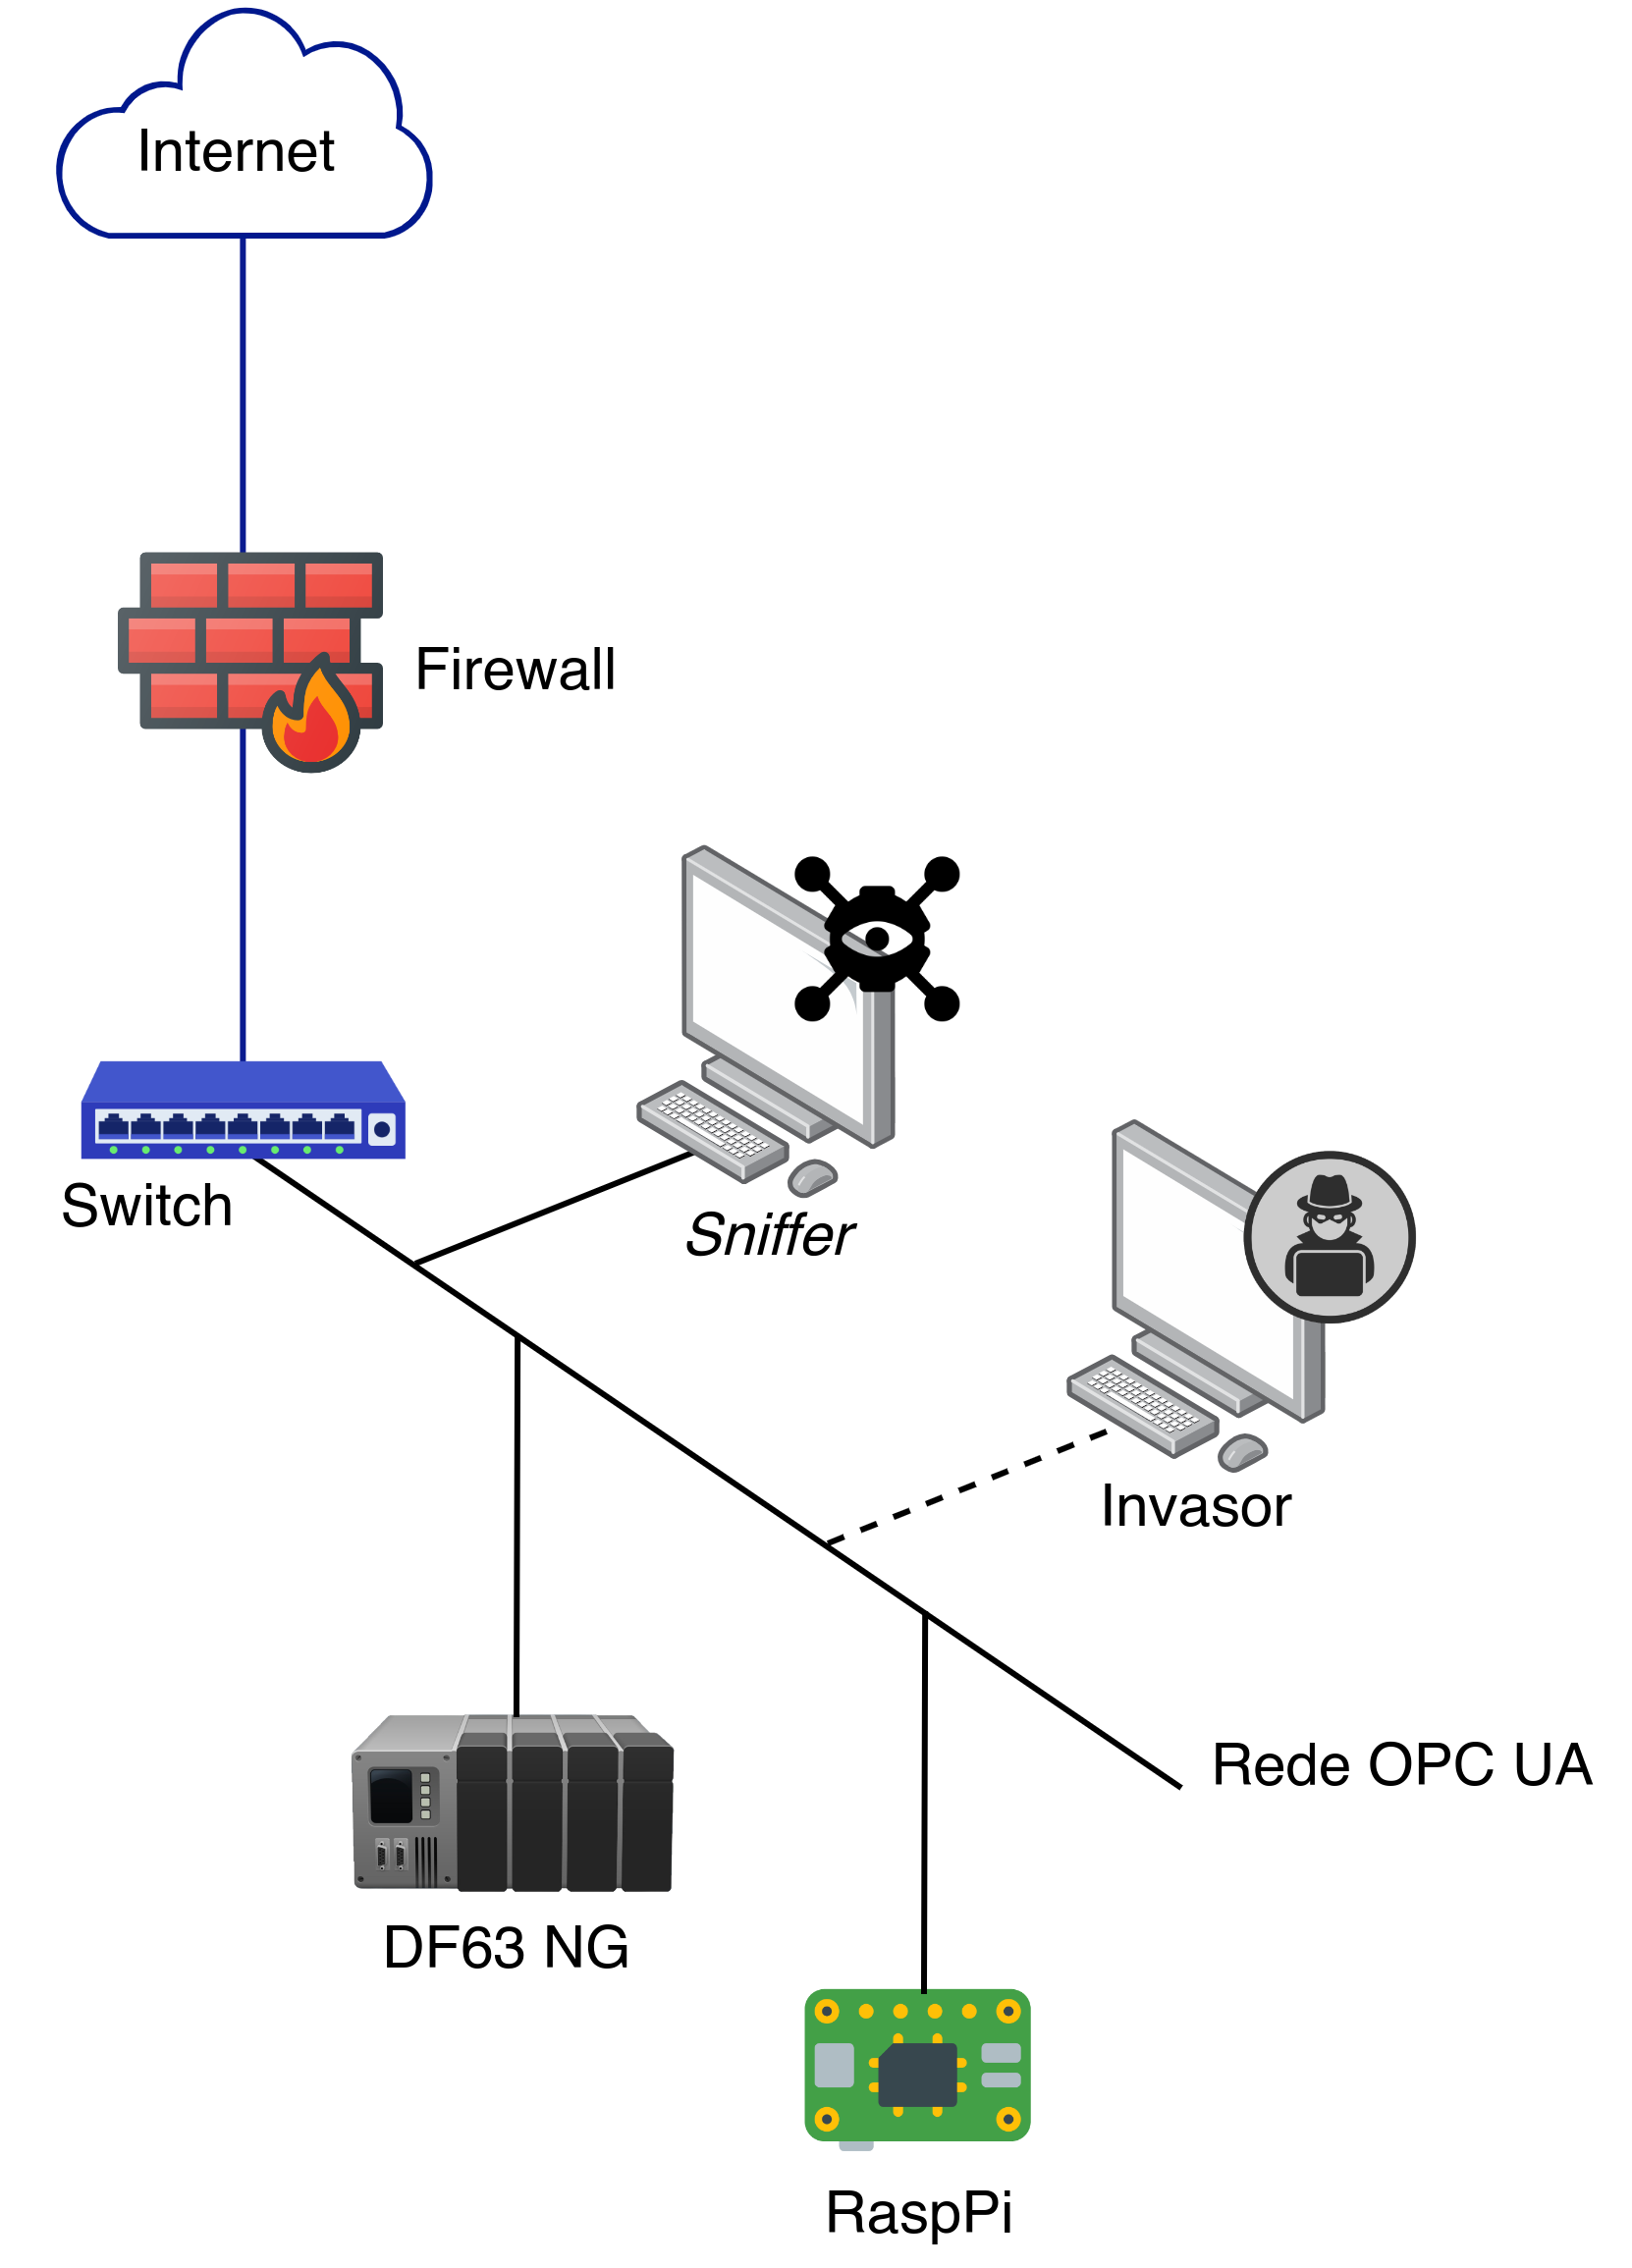
\includegraphics[width=0.6\textwidth]{USPSC-img/bancada.png}
        \end{center}
        \legend{Fonte: elaborada pelo autor.}
    \end{figure}

    \subsection{\textit{Hardware}}

        Para simular os ataques cibernéticos, é necessário um conjunto de componentes de \textit{hardware} combinado com ferramentas de \textit{software} específicas. A seguir, são detalhados os equipamentos utilizados.

        \begin{itemize}
            \item \underline{DF63 NG}: representa a nova geração de controladores multifuncionais da plataforma DFI302 da Nova Smar S/A, funcionando como um `\textit{linking device}' para conectar redes H1 independentes e redes Ethernet HSE. Foi especialmente projetado para soluções de controle distribuído em redes industriais. Além de suportar comunicação Modbus, oferece recursos avançados, incluindo redundância `\textit{Hot standby}', comunicação OPC UA nativa, estampa de tempo e configuração por meio da linguagem Ladder conforme IEC 61131. A DF63 NG é altamente versátil, permitindo a instanciação de centenas de blocos funcionais, incluindo blocos flexíveis, e possui um servidor Web integrado para diagnóstico e parametrização;
            \item \underline{Raspberry Pi 4 Modelo B}: é utilizado um mini-computador de placa única multiplataforma, configurado com o sistema operacional Kali Linux, hospedando um servidor OPC UA. A Raspberry Pi 4 Modelo B representa uma evolução significativa em relação às gerações anteriores, incorporando um processador ARM Cortex-A72 quad-core de 64 bits, rodando a 1,5 GHz, suporte a Wi-Fi 802.11ac, Bluetooth 5.0 e maior capacidade de memória. Estes aprimoramentos garantem um ambiente experimental mais robusto e uma capacidade de processamento aprimorada para a condução de testes de intrusão em redes OPC UA;
            \item \underline{Ethernet Switch}: trata-se de um dos dispositivos de rede mais ubíquos, empregado para centralizar a comunicação entre múltiplos dispositivos. Utiliza a técnica de comutação de pacotes para receber e encaminhar dados de um dispositivo para outro. Neste projeto, faz-se uso de um \textit{switch} Ethernet da marca TP-Link para estabelecer uma conexão entre os clientes OPC UA e o servidor. O componente de rede que atua como hospedeiro do servidor OPC UA está conectado ao comutador Ethernet por meio de um cabo LAN, da mesma maneira que outro responsável por hospedar o cliente também está conectado ao \textit{switch}. Cumpre destacar que os comutadores Ethernet da TP-Link incorporam tecnologia Ethernet verde, resultando em economia de consumo energético, enquanto o controle de fluxo IEEE 802.3x proporciona uma transferência de dados confiável;
            \item \underline{Elemento Invasor}: desempenha um papel fundamental na condução dos testes de intrusão propostos neste estudo. Representa uma simulação de ataque por meio de um computador que pode ser configurado de maneira flexível para atender a cenários específicos de teste. Os ataques são realizados utilizando uma variedade de ferramentas de software, como Hping3 e Nmap (veja \autoref{subsec:software}). Vale ressaltar que o Elemento Invasor é empregado com extrema cautela em um ambiente controlado, a fim de evitar qualquer impacto adverso e garantir a segurança contínua. Assim, respeitando rigorosamente as considerações éticas, os ataques efetuados neste trabalho pelo invasor não implicam em nenhuma violação das regulamentações estabelecidas pela Lei Geral de Proteção de Dados (LGPD), por não serem aplicados em nenhuma rede ou implementação real.
        \end{itemize}
    
    \subsection{\textit{Software}} \label{subsec:software}

        Um conjunto de ferramentas de \textit{software} é necessário para conduzir os ataques às redes OPC UA, destacando-se as seguintes:

        \begin{itemize}
            \item \underline{Smar OPC UA server}: servidor OPC UA proprietário da Nova Smar S/A, amplamente aplicado no setor industrial juntamente com a linha de produtos compatíveis com o novo padrão O-PAS (do inglês, \textit{Open Process Automation™ Standards}), desenvolvido pelo OPAF (do inglês, \textit{Open Process Automation™ Forum}). Oferece um ambiente altamente seguro e eficiente para a comunicação e troca de dados em sistemas de automação industrial. A Nova Smar S/A continua aprimorando seu servidor OPC UA para atender às crescentes demandas do mercado, proporcionando uma solução de conectividade sólida e confiável;
            \item \underline{opcua-asyncio}: implementação de código aberto do OPC UA, escrita em Python com suporte para asyncio. Opera sob a GNU Lesser General Public License v3.0, permitindo sua integração e distribuição com \textit{software} proprietário. Essa biblioteca é versátil, compatível com vários ambientes Python, e oferece informações detalhadas sobre a implementação de clientes e servidores OPC UA. O opcua-asyncio implementa o conjunto de protocolos binários OPC UA, SDK de cliente e servidor, e é uma opção flexível para desenvolvedores que preferem Python como linguagem de programação;
            \item \underline{OPC UA Exploit Framework}: projeto \textit{open-source} desenvolvido e mantido pela Claroty Team82, que fornece um framework avançado de ferramentas para pesquisa e exploração de vulnerabilidades em redes OPC UA. O intuito deste projeto é facilitar e auxiliar empresas desenvolvedoras de software e fornecedoras de OPC UA na fase de teste e aprimoramento de seus produtos, além de suportar pesquisadores da área na análise de novas vulnerabilidades e \textit{bugs} sistêmicos;
            \item \underline{Ettercap}: ferramenta de \textit{software} utilizada principalmente para implementar ataques do tipo MITM. Possui recursos extras de captura de conexões em \textit{real-time}, filtragem de conteúdo e análise de \textit{hosts} de destino. O Ettercap é utilizado neste projeto para implementar o primeiro cenário de ataque, capturando a conexão entre cliente e servidor OPC UA;
            \item \underline{Hping3}: ferramenta de linha de comando que serve como montadora e analisadora de pacotes TCP/IP. Inicialmente concebida para executar ataques de negação de serviço (DoS), o Hping3 é agora amplamente empregado em testes de segurança de rede. Oferece suporte a protocolos TCP, UDP e ICMP, bem como um modo de rastreamento de rota;
            \item \underline{Wireshark}: \textit{software} de código aberto usado para capturar e analisar pacotes e protocolos de rede. É principalmente aplicado para solução de problemas de rede, desenvolvimento e análise de protocolos de \textit{software} e comunicação. Neste trabalho, é utilizado juntamente com um computador \textit{sniffer};
            \item \underline{Nmap}: ferramenta gratuita de código aberto amplamente utilizada para varredura de rede e portas. Através dela, pode-se descobrir os \textit{hosts} e serviços em uma rede, bem como detalhes como qual serviço está em execução em qual porta e se a porta está aberta ou fechada, entre outros. Esse resultado é alcançado ao enviar pacotes para o alvo e analisar posteriormente sua resposta.
        \end{itemize}

\section{Ataques Cibernéticos em Redes Industriais OPC UA} \label{sec:attacks}

    Nesta seção, é apresentada uma análise detalhada dos cenários de ataque implementados minuciosamente neste projeto. A exposição abrange uma descrição passo a passo das metodologias empregadas para orquestrar três formas distintas de ciberataques: interceptação de pacotes (\textit{Packet Sniffing}), ataques do tipo MITM e negação de serviço. Ao elucidar as complexidades desses vetores de ataque, objetiva-se proporcionar uma compreensão profunda do cenário em evolução das ameaças à cibersegurança em redes OPC UA.

    \subsection{\textit{Packet Sniffing}}

        Uma vez que a rede OPC UA esteja instalada e funcionando em seus respectivos dispositivos, o Elemento Invasor inicia o \textit{software} Ettercap, utilizando-o como um \textit{sniffer} unificado para obter informações detalhadas sobre os alvos disponíveis na rede. O modo unificado do Ettercap permite a execução do ataque por meio de uma única interface de rede. É importante observar que o Elemento Invasor deve estar configurado na mesma rede de comunicação OPC UA e conectado a uma porta do \textit{switch} gerenciável, que, por sua vez, replica o tráfego de dados das outras portas (do componente cliente e servidor OPC UA), conforme ilustrado na \autoref{fig:sniffing}.

        \begin{figure}[htbp]
            \caption{\label{fig:sniffing}Esquemático do ataque \textit{Packet Sniffing}}
            \begin{center}
                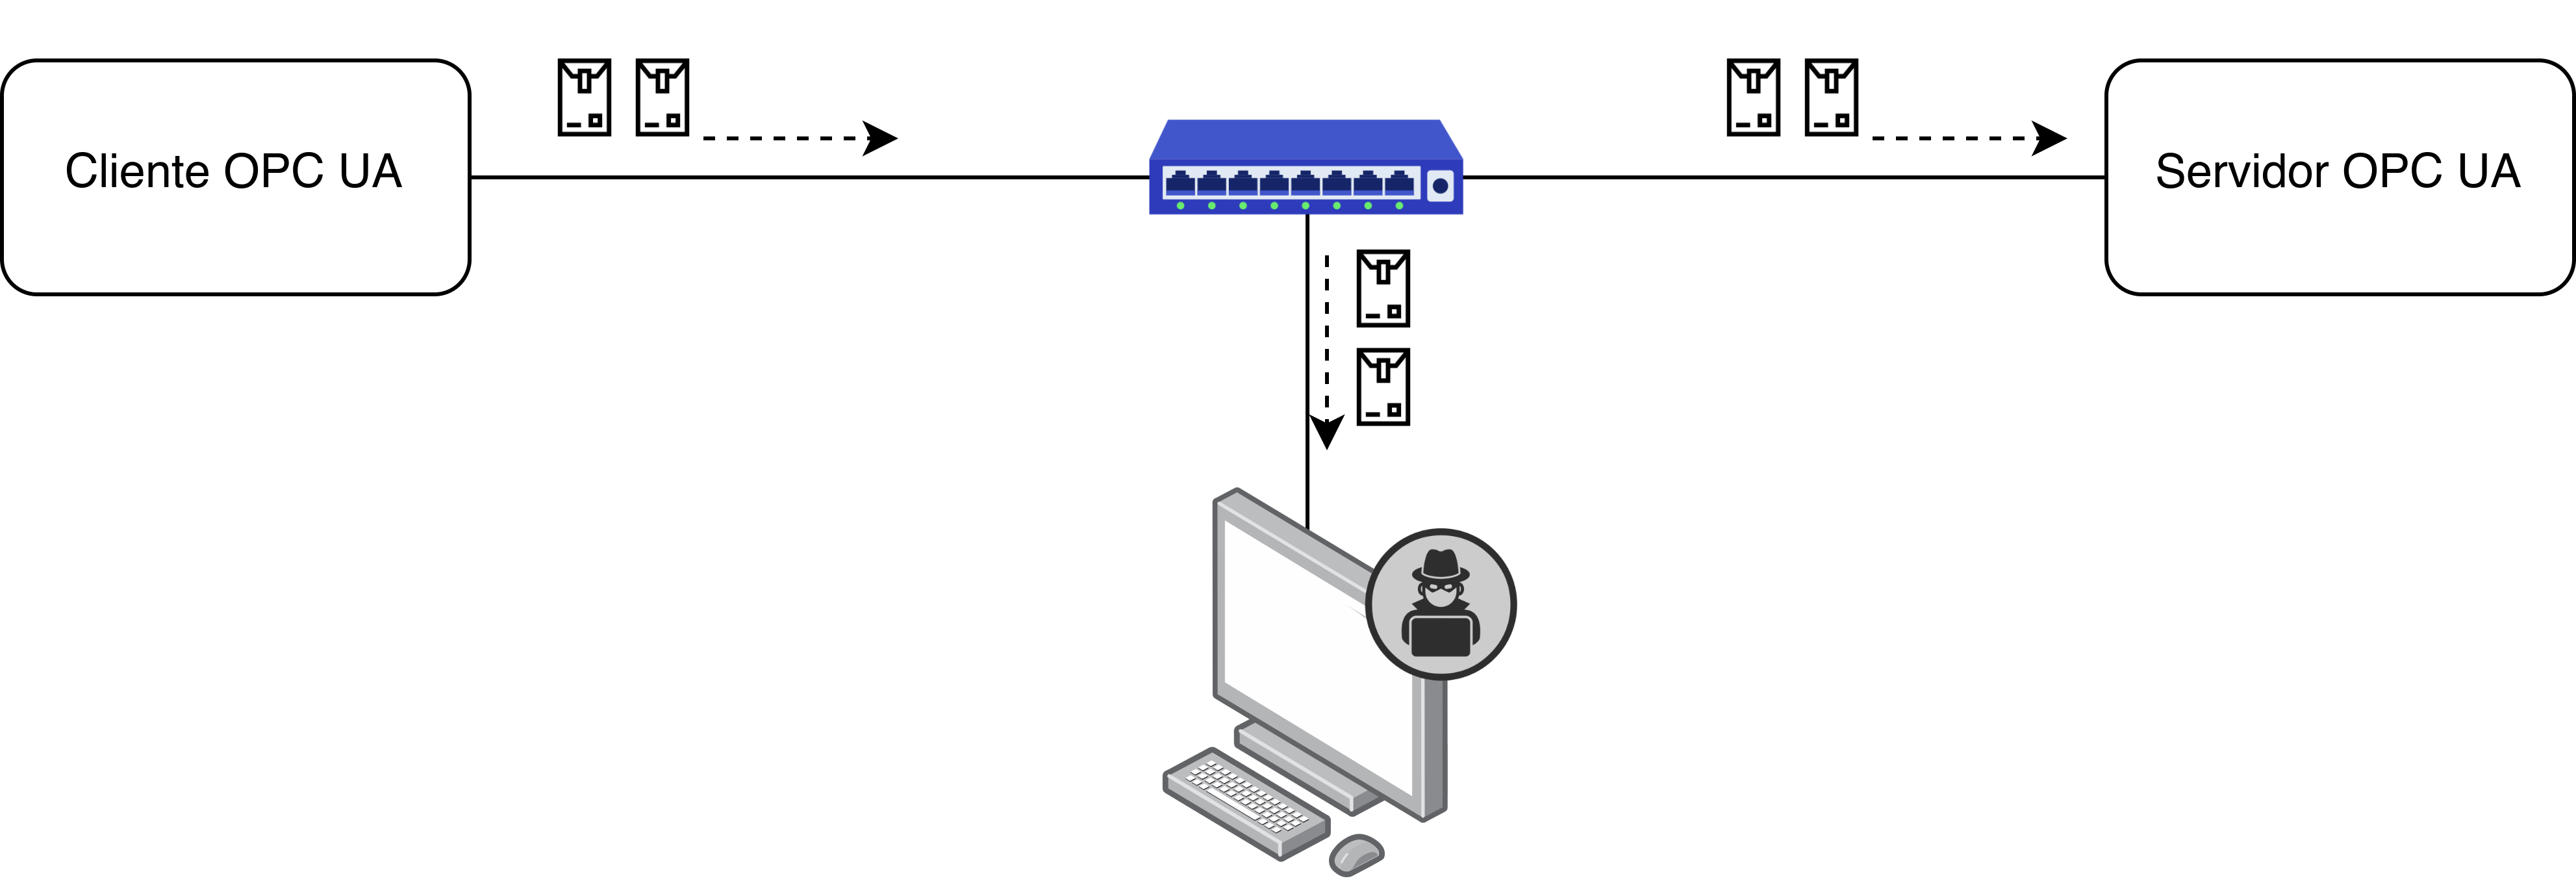
\includegraphics[width=0.9\textwidth]{USPSC-img/sniffing.png}
            \end{center}
            \legend{Fonte: elaborada pelo autor.}
        \end{figure}
        
        Com o \textit{sniffing} de rede iniciado pelo Ettercap, utiliza-se o Wireshark para analisar mais detalhes sobre os endereços obtidos. A \autoref{fig:sniffWire} apresenta a série de pacotes que o \textit{software} disponibiliza quando a operação de \textit{sniffing} do tráfego de rede é bem-sucedida. Maiores detalhes da análise aplicada aos dados obtidos nesse processo são apresentados no \autoref{cap:resultados}.

        \begin{figure}[htbp]
            \caption{\label{fig:sniffWire}Resultados de captura do Wireshark durante o \textit{sniffing} de pacotes}
            \begin{center}
                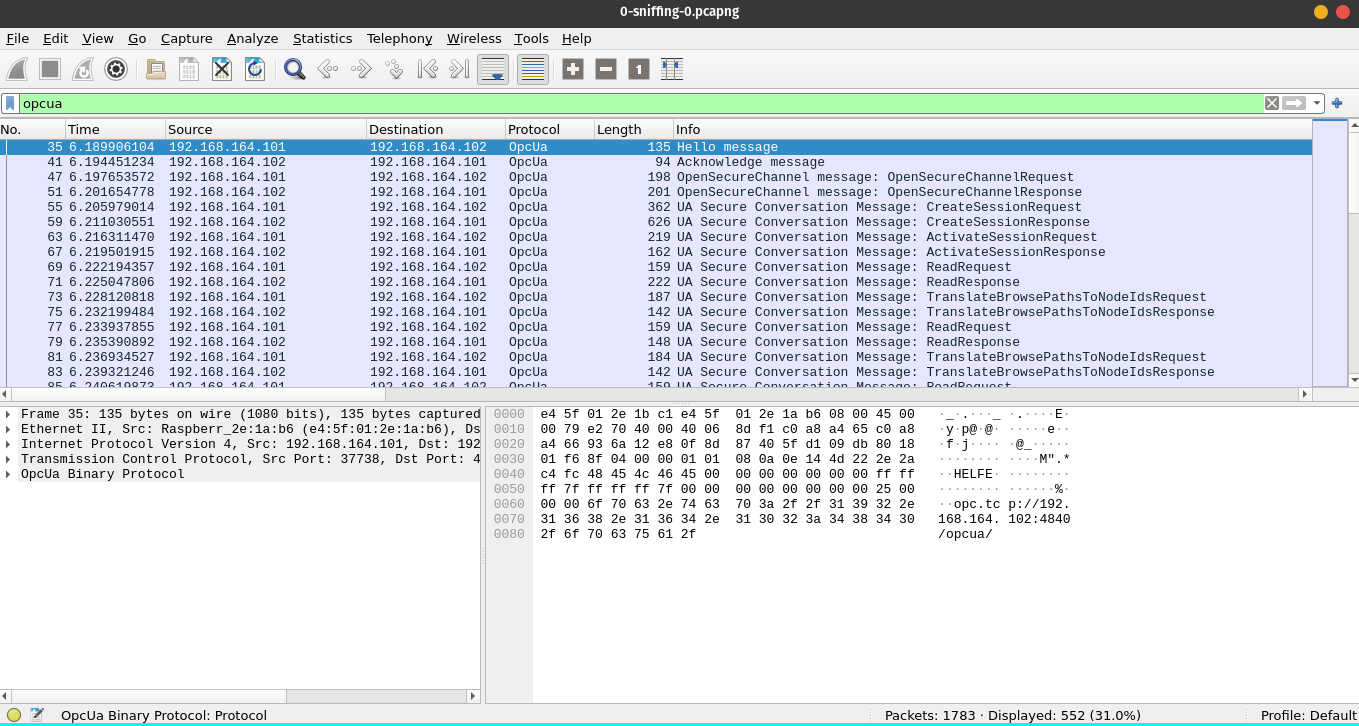
\includegraphics[width=1\textwidth]{USPSC-img/sniffWire.png}
            \end{center}
            \legend{Fonte: elaborada pelo autor.}
        \end{figure}
        
        Os detalhes dos pacotes capturados pelo Wireshark são analisados e descritos minuciosamente no \autoref{cap:resultados}.
    
    \subsection{\textit{Man in the Middle (MITM)}}

        Ao realizar esse ataque, o Elemento Invasor pode interceptar as informações do \textbf{SecureChannel} entre o cliente e o servidor OPC UA, como mostra a \autoref{fig:mitm}.

        \begin{figure}[htbp]
            \caption{\label{fig:mitm}Esquemático do ataque MITM}
            \begin{center}
                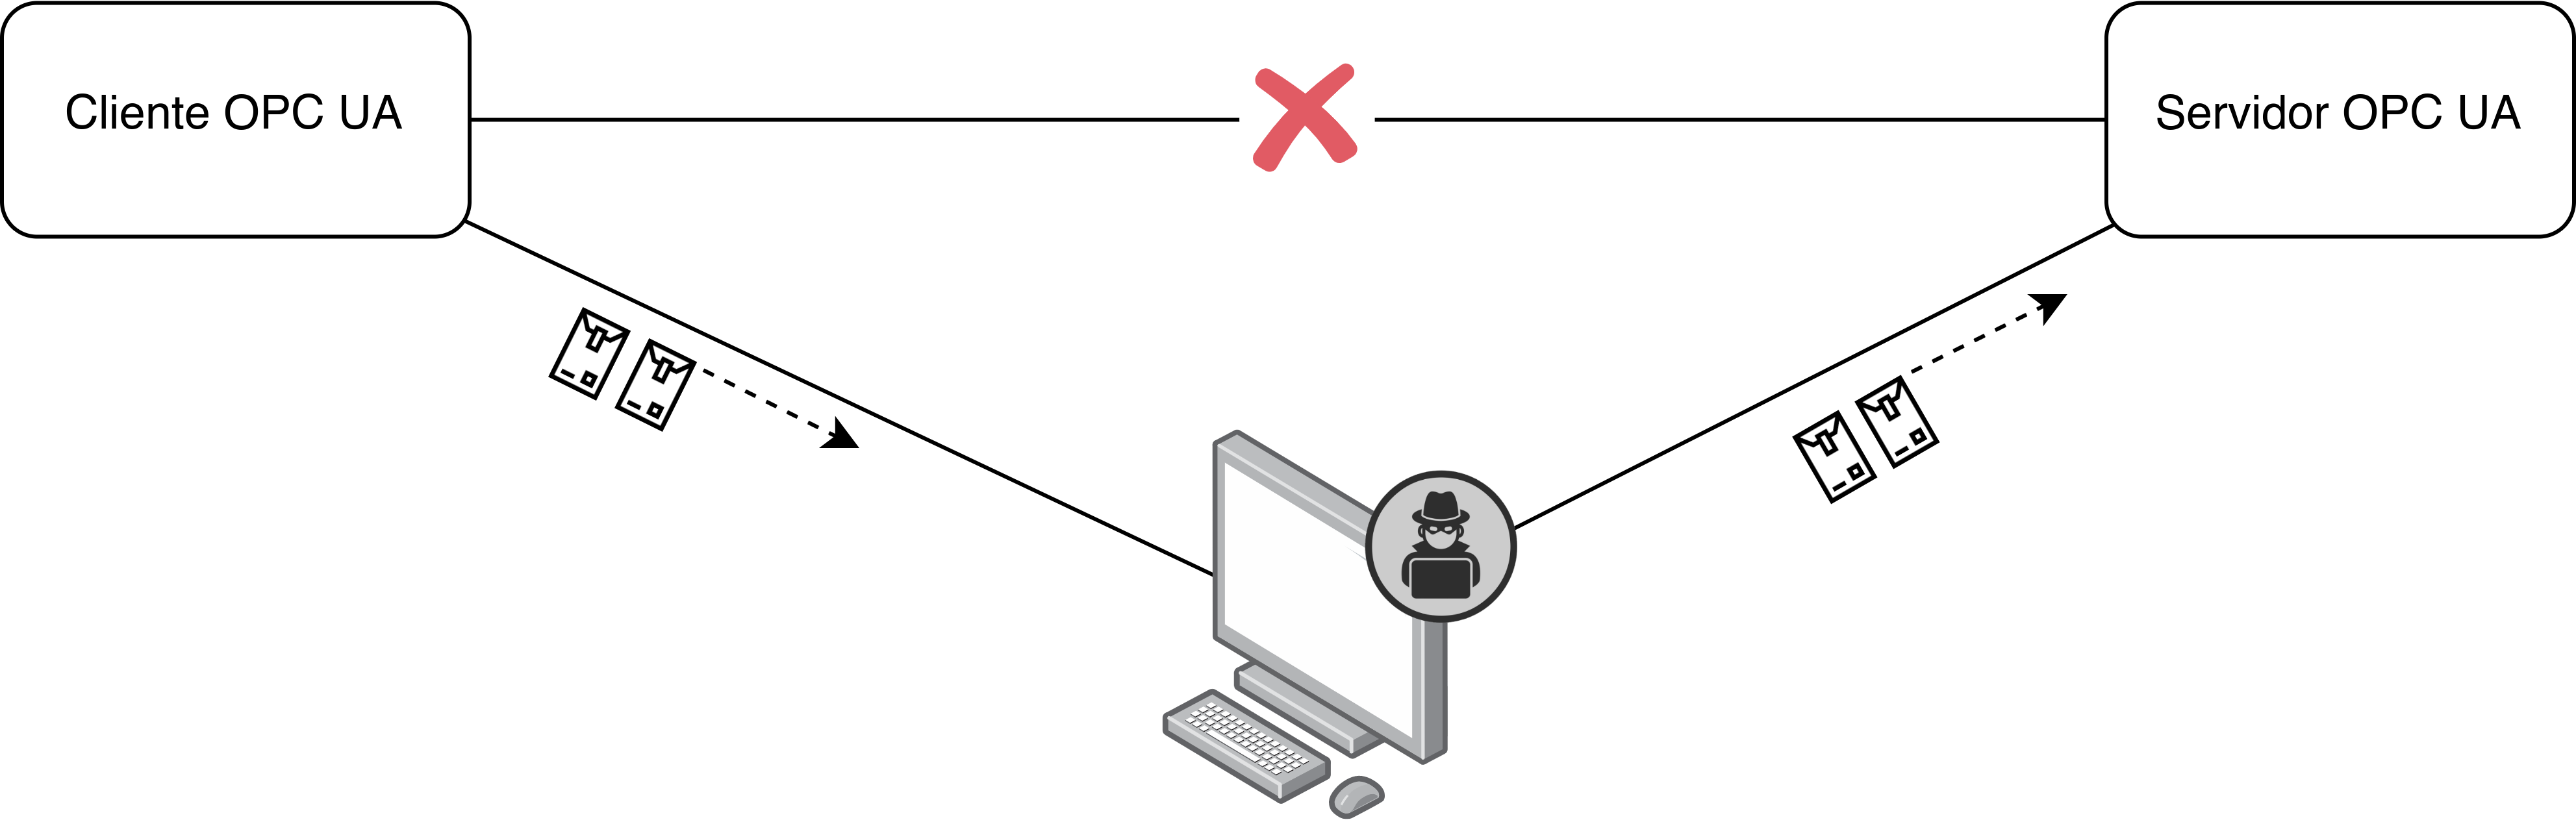
\includegraphics[width=0.9\textwidth]{USPSC-img/mitm.png}
            \end{center}
            \legend{Fonte: elaborada pelo autor.}
        \end{figure}
        
        A primeira ferramenta de software utilizada nesse processo é o Ettercap, empregada para realizar uma varredura da rede. Ao iniciar a busca direta por \textit{hosts} ativos, todos os endereços da máscara de rede são verificados a fim de identificar quais estão em funcionamento. Por exemplo, caso a máscara de rede configurada seja 255.255.255.0 (24), um total de 256 endereços são varridos.
        
        Após o término dessa operação de varredura, o Elemento Invasor pode selecionar os alvos que receberão o ataque MITM e, então, prosseguir com a falsificação da rede por ARP (do inglês \textit{ARP Spoofing}), um dos métodos mais comuns para efetuar esse ataque. O ARP (do inglês \textit{Address Resolution Protocol}) é um dos protocolos de comunicação mais importantes da camada de rede do modelo OSI, utilizado para determinar o endereço MAC (do inglês \textit{Media Access Control}) de um dispositivo com base no seu endereço IP. Com o \textit{ARP Spoofing}, o invasor é capaz de anunciar à rede que o seu endereço MAC é o correto para os endereços IP pertencentes ao roteador e à estação de trabalho. Assim, esses dois dispositivos atualizam as suas entradas de cache ARP e, a partir desse ponto, comunicam-se com o invasor, em vez de diretamente entre si.

        Além disso, realizou-se também o ataque MITM por roubo de portas (do inglês \textit{port stealing}) com a ferramenta Ettercap. Neste cenário, o invasor intercepta o tráfego de rede entre o cliente e o servidor OPC UA ao inundar a rede com pacotes ARP, cujo endereço MAC de destino é o do próprio invasor e o endereço MAC de origem é o de uma vítima. Com isso, a porta do switch do alvo é ``roubada'', permitindo que os pacotes destinados a ela sejam recebidos pelo invasor. O invasor então interrompe a inundação, realiza uma solicitação ARP para o destino real do pacote e, ao receber a resposta, reenvia o pacote para o destino. O processo é repetido continuamente para interceptar o tráfego.

        Enquanto os ataques MITM por falsificação da tabela ARP e por roubo de portas são realizados pela ferramenta Ettercap, inicia-se a captura de pacotes pelo Wireshark. Para facilitar a visualização e a análise realizada neste estudo, o Wireshark é configurado para o protocolo OPC UA, permitindo um exame detalhado da comunicação entre os dispositivos na rede.
    
    \subsection{\textit{Denial of Service (DoS)}}

        Esse tipo de ataque possibilita a inserção de clientes não confiáveis na rede OPC UA pelo Elemento Invasor, assim como uma inundação da rede e do servidor ao enviar mensagens específicas continuamente. A \autoref{fig:dos} apresenta um esquema básico do funcionamento de um ataque DoS, no qual as solicitações advindas de um cliente OPC UA não confiável são interpretadas pelo servidor, mas não aceitas devido à falsificação de endereço.

        \begin{figure}[htbp]
            \caption{\label{fig:dos}Esquemático do ataque DoS}
            \begin{center}
                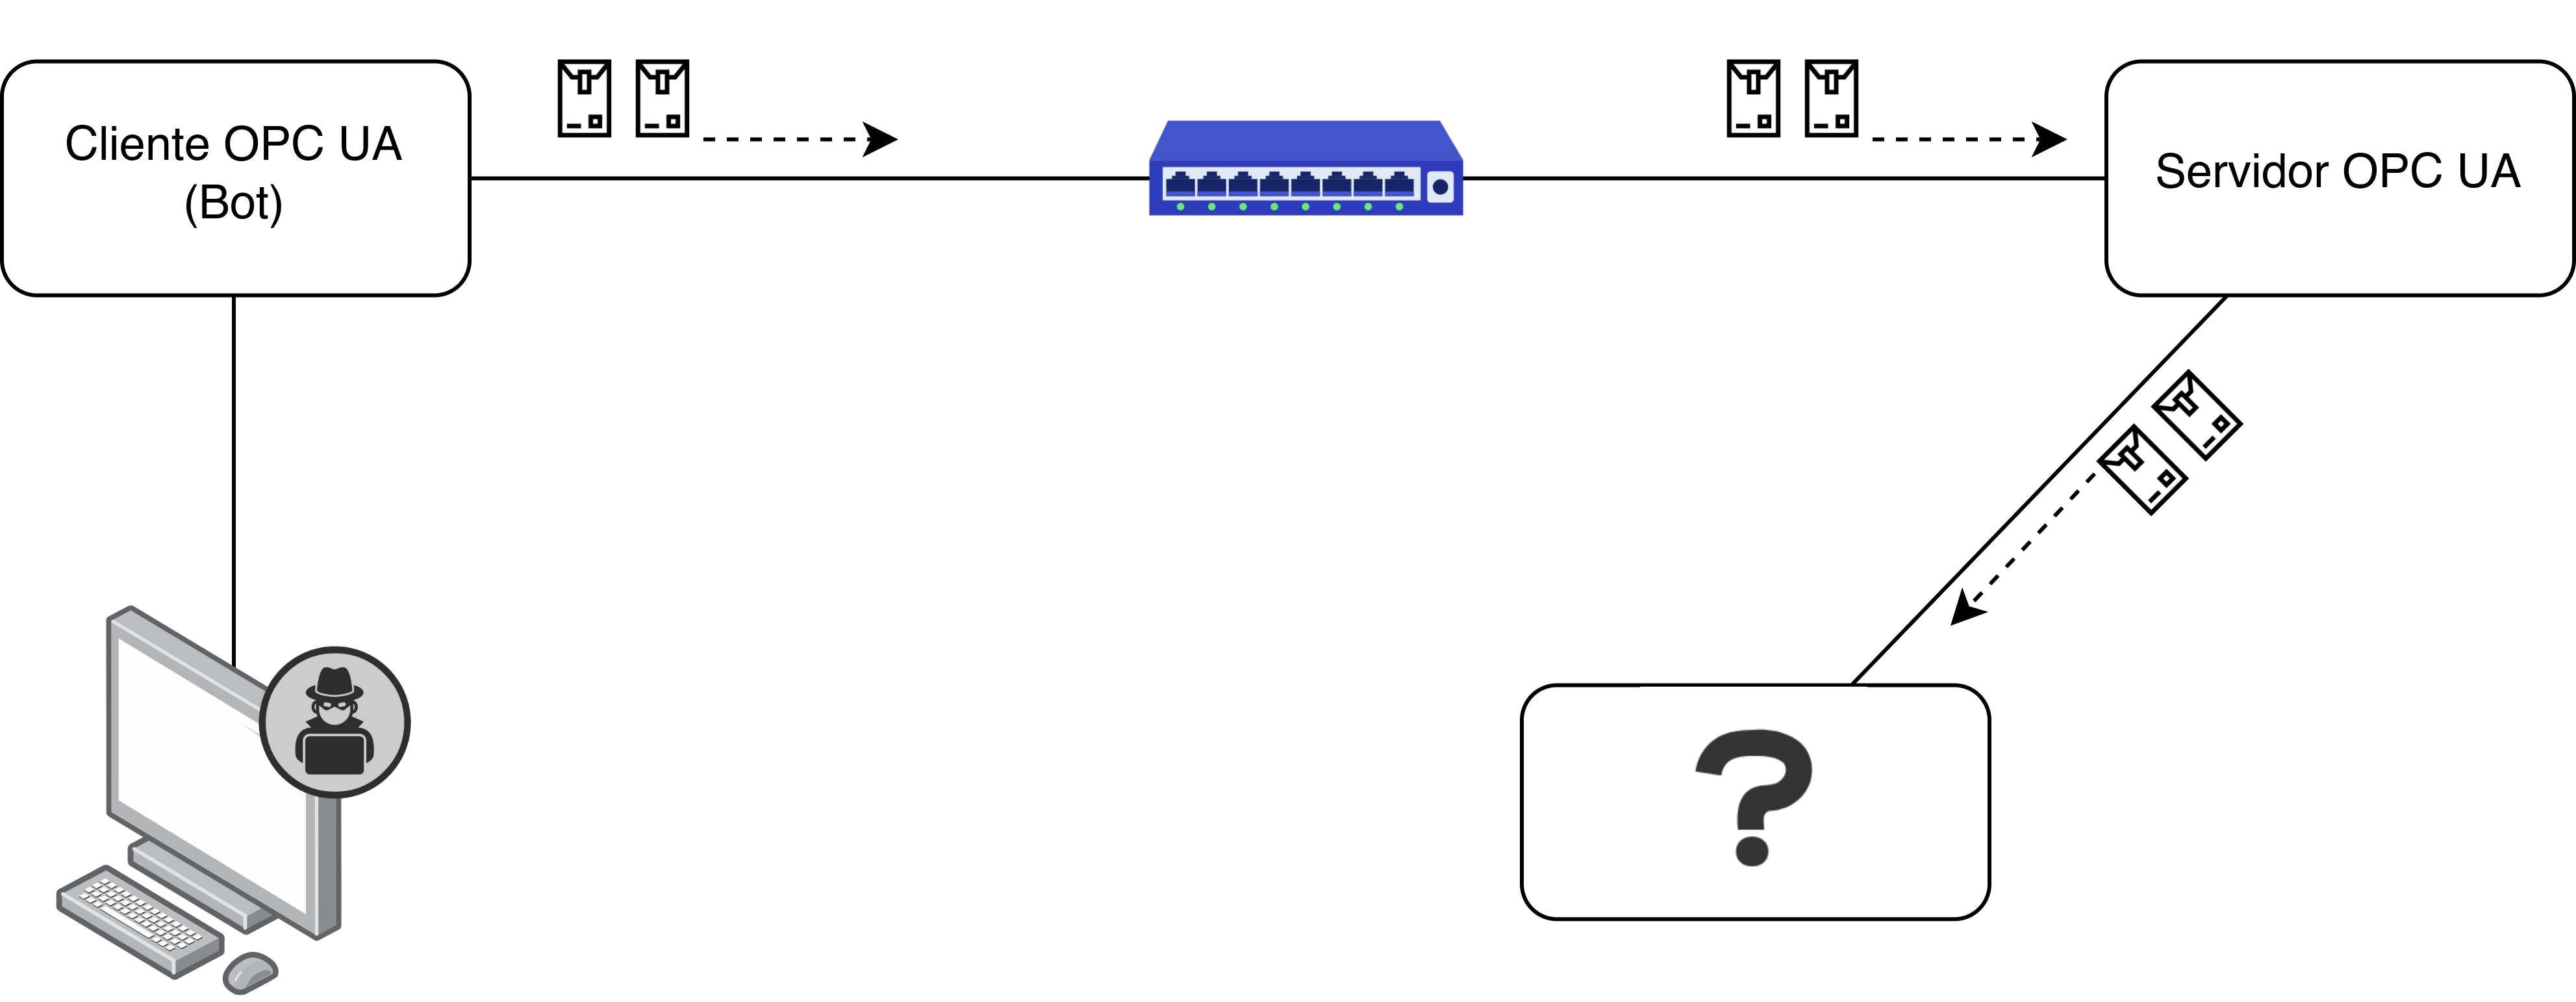
\includegraphics[width=0.9\textwidth]{USPSC-img/dos.png}
            \end{center}
            \legend{Fonte: elaborada pelo autor.}
        \end{figure}
        
        Existem diversos cenários possíveis para a efetuação do ataque de negação de serviço. Além do impacto da inundação na rede, ressaltam-se os efeitos no processamento do componente ao sofrer ataques intensivos, nos quais o servidor precisa avaliar as certificações para responder às solicitações. Segundo \citeonline{neu2019}, os principais cenários são:

        \begin{enumerate}
            \item \underline{SYN \textit{Flooding}}: o cliente sobrecarrega o servidor enviando mensagens SYN de forma contínua, e o servidor responde com mensagens ACK a cada uma delas. Embora essa ação possa inundar a rede com tráfego sobrecarregado, seu impacto no consumo de recursos do servidor é limitado;
            \item \underline{ACK ou ERR \textit{Flooding}}: nesse cenário, o cliente inunda o servidor com mensagens ACK e/ou ERR, às quais o servidor responde com mensagens ERR. Assim como no caso anterior, pode haver sobrecarga na rede, mas o impacto nos recursos do servidor é moderado;
            \item \underline{Inundação com Mensagens Incorretas}: o Elemento Invasor envia continuamente mensagens incorretas, forçando o servidor a responder com mensagens ERR. Isso também gera sobrecarga na rede, mas o impacto no processamento do servidor é relativamente baixo;
            \item \underline{CLO \textit{Flooding}}: mensagens de solicitação de fechamento de canal (CLO) são enviadas repetidamente ao servidor, que responde com mensagens ERR, sobrecarregando a rede com esse tráfego;
            \item \underline{Inundação com \textbf{FindServers} ou \textbf{GetEndpoints}}: o cliente estabelece um canal no modo de segurança `None' e, em seguida, envia continuamente mensagens \textbf{FindServers()} ou \textbf{GetEndpoints()} para o servidor, que responde utilizando o protocolo OPC UA MSG. Embora haja impacto na rede, não há alteração significativa nos recursos do servidor;
            \item \underline{Inundação com Solicitações SYN e OPN}: um cliente não confiável realiza um ataque de negação de serviço enviando continuamente solicitações SYN e OPN ao servidor, que responde com mensagens ACK e ERR. Nesse ataque, o servidor consome recursos substanciais durante a validação do certificado, na solicitação e no processo de criptografia da mensagem. Esse ataque pode ser ainda mais eficaz quando a Autoridade de Certificação está localizada em um sistema diferente, aumentando consideravelmente o tempo de validação do certificado e, consequentemente, o processamento do componente onde se encontra o servidor.
        \end{enumerate}

        Duas ferramentas são utilizadas para efetuar a inundação da rede e, assim, alcançar o DoS: OPC UA Exploit Framework e Hping3. Além disso, o Nmap é aplicado para realizar uma varredura da rede com o objetivo de encontrar portas abertas e endereços IP disponíveis.

        Uma vez que o Elemento Invasor obtém acesso a algum dos componentes da rede do alvo, o Nmap é utilizado para o mapeamento da rede. O comando abaixo executa um \textit{scan} SYN em um intervalo de IPs, sendo relativamente não intrusivo e camuflado, pois nunca completa uma conexão TCP. Também conhecido como escaneamento de portas entreabertas (\textit{half-open scanning}), um pacote SYN é enviado como se fosse abrir uma conexão real, para a qual se espera uma resposta. Um SYN/ACK indica que a porta está ativa (aberta), enquanto um RST (\textit{reset}) sugere que a porta não está ativa. Se nenhuma resposta é recebida após várias retransmissões, a porta é marcada como filtrada. A porta também é considerada filtrada se um erro ICMP de inalcançável for recebido.

        \begin{minted}[
            breaklines,
            %linenos,
            mathescape,
            encoding=utf8,
            framesep=2mm,
            baselinestretch=1.2,
            bgcolor=codeback,
            fontsize=\footnotesize
        ]{console}
nmap -sS 192.168.164.*
        \end{minted}

        A execução correta desse mapeamento resulta em uma lista de IPs disponíveis e portas abertas, que servirão como base para os próximos passos. O Hping3 é utilizado para realizar o SYN \textit{Flooding} (1) na rede. Para isso, o \textit{script} de configuração abaixo deve ser implementado pelo Elemento Invasor, customizando-o conforme o cenário específico.

        \begin{minted}[
            breaklines,
            %linenos,
            mathescape,
            encoding=utf8,
            framesep=2mm,
            baselinestretch=1.2,
            bgcolor=codeback,
            fontsize=\footnotesize
        ]{bash}
# CONFIGURAÇÃO
set TARGET "192.168.164.101"  # O alvo do ataque
set FAKEIP "192.168.164.201"  # Endereço falso
set BROADCAST "192.168.164.254"  # Endereço de broadcast da rede

set PORTS {{4840}{4192}}  # Utilizar as portas abertas encontradas no Nmap
set PORTUDP 123  # Utilizar uma porta UDP ativa

set commandRunTime 60

# EXECUÇÃO
foreach port $PORTS {
    lappend commands "hping3 -S -a $FAKEIP -p $port --flood -V $TARGET"
}
        \end{minted}

        Com o \textit{script} configurado, o Hping3 está preparado para iniciar o ataque direcionado ao endereço e às portas especificadas, com uma frequência predefinida (neste caso, sessenta segundos). A interpretação dos parâmetros utilizados na execução é a seguinte: o argumento \textbf{-S} define o tipo de ataque; \textbf{-p} identifica a porta de destino; \textbf{-V} indica o endereço IP do alvo; enquanto \textbf{-a} determina o endereço IP falsificado utilizado no ataque, uma estratégia que pode contornar \textit{firewalls} de forma eficaz.

        Por fim, alguns ataques mais robustos são executados com o auxílio da ferramenta OPC UA Exploit Framework. Os ataques de negação de serviço disponibilizados pelo \textit{framework}, selecionados para execução no ambiente de simulação industrial proposto, são apresentados abaixo, seguidos de suas respectivas categorias, conforme os cenários mencionados e descritos por \citeonline{neu2019}:

        \begin{itemize}
            \item[N/A] \underline{Loop infinito na cadeia de certificados}: refere-se a uma situação em que um servidor implementa a verificação da cadeia de certificados por conta própria, sem proteção contra um loop infinito. Isso pode ocorrer quando, por exemplo, o certificado A é assinado por um certificado B, que, por sua vez, é assinado pelo certificado A. Cria-se, assim, uma dependência circular entre os certificados A e B, resultando em um loop infinito durante o processo de verificação da cadeia de certificados;
            % \item[(3)] \underline{Inundação por \textit{Chunk}}: envolve o envio de uma quantidade abundante de fragmentos de dados ao servidor sem o envio do fragmento final correspondente. O OPC UA permite a divisão dos dados em fragmentos, comumente chamados como \textit{MessageChunks} ou \textit{Chunks}, que são enviados à medida que são codificados, a fim de facilitar a transmissão e o processamento. Caso ocorra um erro na criação de um destes fragmentos, um \textit{Chunk} final deve ser enviado ao destinatário para notificar o erro, que por sua vez, é marcado com um sinalizador `A' (abortar) para indicar o erro. O receptor deve verificar a segurança do \textit{MessageChunk} abortado antes de processá-lo e, caso esteja tudo certo, ignorar a mensagem, mas sem encerrar o \textbf{SecureChannel};
            \item[(3)] \underline{Chamada da função \textit{Dereference} nula}: envolve a chamada de vários métodos OPC UA, seguida pelo encerramento da sessão antes da conclusão desses métodos. Isso resulta em uma situação em que a aplicação servidora é forçada a referenciar um objeto nulo ou um ponteiro inválido, levando a um erro de execução;
            \item[(6)] \underline{Abertura de múltiplos canais seguros}: tentativa de inundar o servidor com um grande número de solicitações \textbf{OpenSecureChannels};
            % \item[(3)] \underline{Mensagem aninhada complexa}: aplicação de uma variante especialmente manipulada e complexa, projetada para explorar vulnerabilidades em um servidor OPC UA. Quando esta variante é processada pelo servidor, ela pode causar um estouro na pilha de chamadas (\textit{call stack overflow}), levando a uma falha no servidor;
            \item[(5)] \underline{Tradução do caminho de navegação}: são enviadas ao servidor requisições de traduções de \textit{browse paths} complexos que exploram a falta de limites adequados na resolução desses caminhos, podendo também causar um \textit{call stack overflow}.
            % \item[Não aplicável] \underline{Falha de espera no \textit{Thread Pool}}: caracteriza uma paralisação (\textit{deadlock}) no sistema de \textit{Thread Pool} -- mecanismo de gerenciamento de \textit{threads} utilizado para processar solicitações de clientes e tarefas no servidor OPC UA -- devido à inanição simultânea de tarefas concorrentes. Em termos mais simples, quando vários processos ou \textit{threads} estão competindo por recursos do \textit{Thread Pools} de um servidor e, devido a problemas de sincronização ou gerenciamento inadequado de \textit{threads}, ficam em um estado de espera prolongado, impedindo efetivamente o servidor de processar solicitações legítimas;
            % \item[(6)] \underline{Persistência ilimitada de subscrições}: inúmeras solicitações de monitoramento ao servidor são enviados por um invasor, todas configuradas para não excluir os itens após o monitoramento. Esta persistência resulta em uma alocação descontrolada de recursos de memória pelo servidor, levando eventualmente a uma negação de serviço devido ao esgotamento de recursos.
            % \item[(3)] \underline{Chamada da função \textit{Dereference} nula}: envolve a chamada de vários métodos OPC UA e encerramento da sessão antes da conclusão destes. Isso resulta em uma situação em que a aplicação servidora é forçada a referenciar um objeto nulo ou um ponteiro invalido, levando a um erro de execução;
            % \item[(3)] \underline{Alteração de corrida e navegação no espaçamento de endereço}: o Elemento Invasor realiza a adição de \textit{Nodes} no \textit{Address Space} no servidor e, simultaneamente, remove-os em um ciclo contínuo, enquanto percorre todo o espaçamento de endereço. Esta manobra cria uma situação de competição na qual o servidor está sendo constantemente modificado e examinado ao mesmo tempo, podendo, assim, esgotar os recursos de processamento e resultar em problemas de consistência no \textit{Address Space};
            % \item[(6)] \underline{Atualização de condição ilimitada}: refere-se ao envio repetido e quantidade abundante de chamadas do método \textbf{ConditionRefresh}, o que leva a alocações de memória não controladas e, eventualmente, pode resultar em uma falha no sistema. O método ConditionRefresh é usado para atualizar as condições e estados das variáveis monitoradas em um servidor OPC UA.
        \end{itemize}

        Sabendo disso, os ataques mencionados podem ser executados através da seguinte linha de comando base, substituindo SERVER\_TYPE pelo tipo de servidor utilizado (\textit{e.g.}, softing, unified, prosys, kepware, triangle, dotnetstd, open62541, ignition, rust, node-opcua, opcua-python, milo e s2opc), IP\_ADDR pelo endereço IP do alvo, PORT pela porta aberta para a comunicação UA, ENDPOINT\_ADDRESS pelo \textit{endpoint} do servidor, FUNC\_TYPE pelo tipo de ataque escolhido (consultar a documentação oficial do \textit{framework} para verificar os nomes das funções disponíveis \cite{claroty2023}) e DIR, necessário para algumas funções:

        \begin{minted}[
            breaklines,
            %linenos,
            mathescape,
            encoding=utf8,
            framesep=2mm,
            baselinestretch=1.2,
            bgcolor=codeback,
            fontsize=\footnotesize
        ]{console}
python main.py [SERVER_TYPE] [IP_ADDR] [PORT] [ENDPOINT_ADDRESS] [FUNC_TYPE] [DIR*]
        \end{minted}

\section{Metodologia}

    O fluxograma apresentado na \autoref{fig:flux} detalha a sequência e a estrutura das atividades, bem como os passos que compõem a metodologia, posteriormente explicados nas subseções.
    
    \begin{figure}[htbp!]
        \caption{\label{fig:flux}Fluxograma da metodologia proposta}
        \begin{center}
            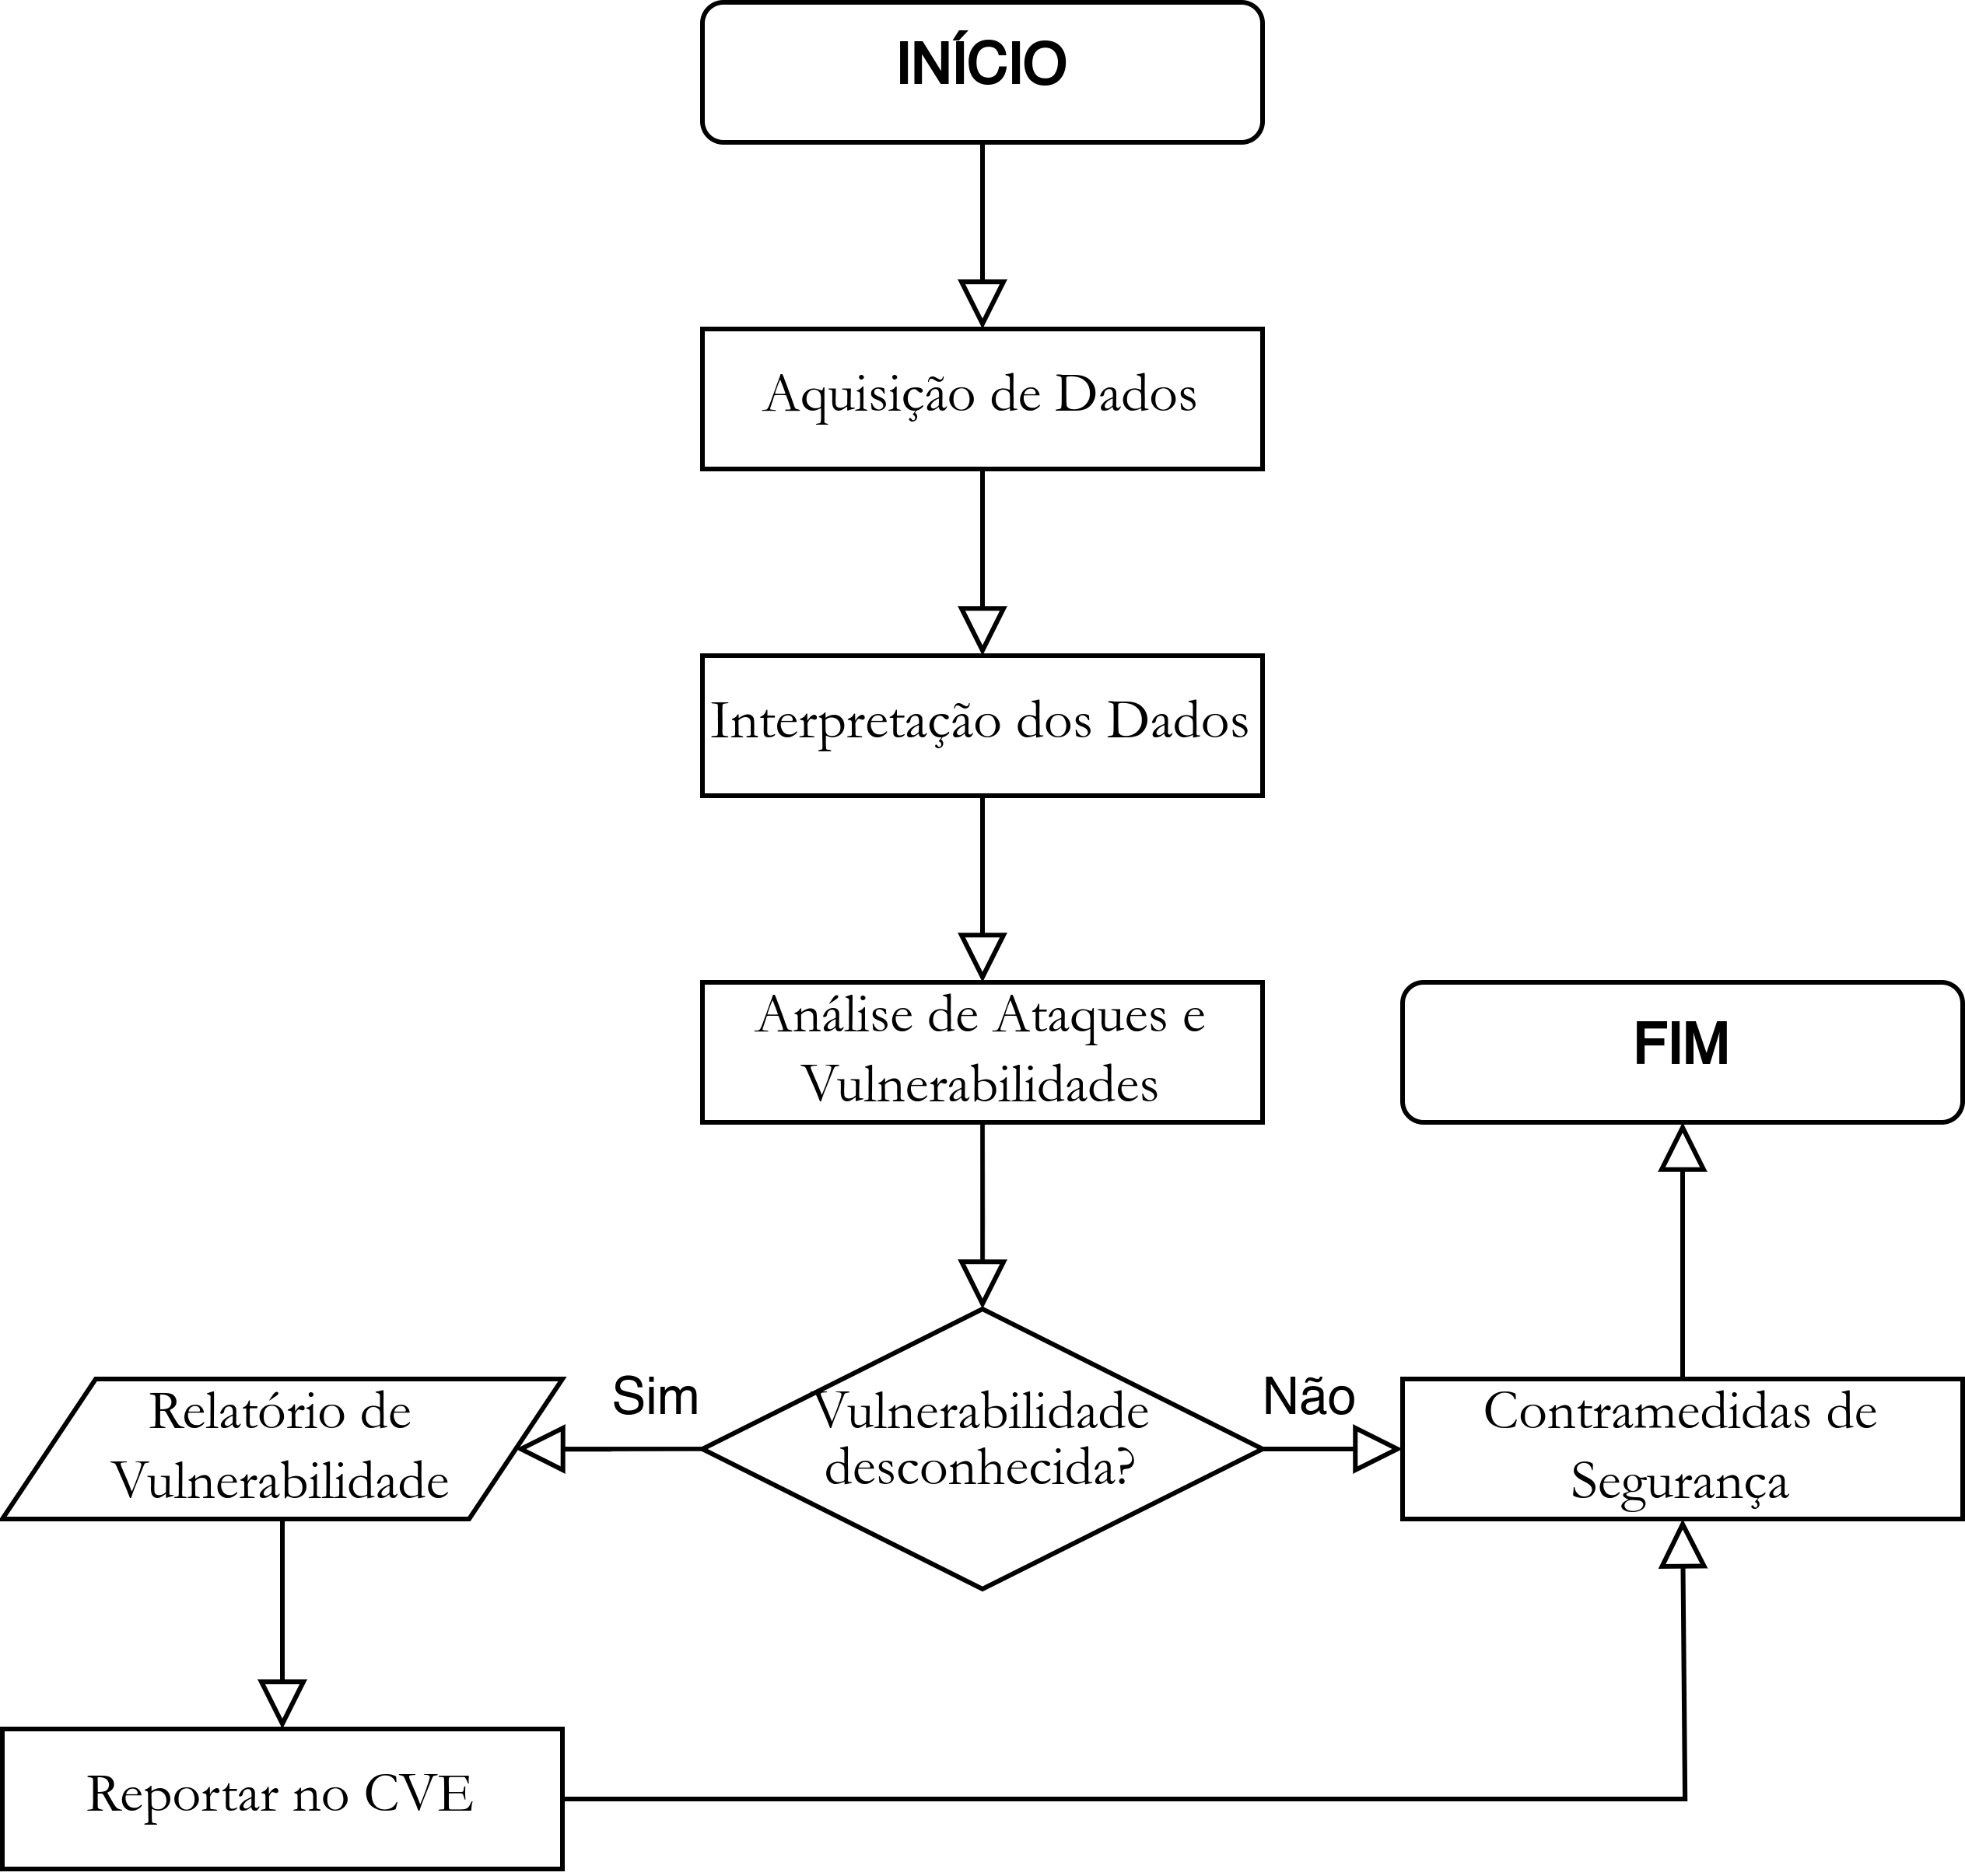
\includegraphics[width=0.7\textwidth]{USPSC-img/fluxograma.png}
        \end{center}
        \legend{Fonte: elaborada pelo autor.}
    \end{figure}

    Para a realização adequada do experimento proposto neste estudo, a infraestrutura de rede do protocolo OPC UA foi configurada conforme os seguintes parâmetros: o Raspberry Pi atuando como servidor e a DF63 NG desempenhando o papel de cliente. Além disso, um elemento de rede denominado \textit{Sniffer} (conforme ilustrado na \autoref{fig:banc}) foi adicionado à configuração para monitorar e registrar a comunicação na rede. Com o objetivo de fornecer uma visão clara dos componentes envolvidos e facilitar a análise dos dados coletados durante o experimento, os endereços IP e MAC de cada elemento do sistema estão resumidos na \autoref{tab:ender}. É importante mencionar que o servidor OPC UA foi configurado para utilizar a porta padrão 4840, e os \textit{endpoints} correspondentes seguem o padrão abaixo. Essa estrutura de configuração foi essencial para a condução eficaz do experimento e a subsequente análise dos resultados.

    \begin{minted}[
        breaklines,
        %linenos,
        mathescape,
        encoding=utf8,
        framesep=2mm,
        baselinestretch=1.2,
        bgcolor=codeback,
        fontsize=\footnotesize
    ]{console}
<esquema>://<endereço>:<porta>/<DiscoveryEndpoint>
    \end{minted}

    Onde, `<esquema>' pode ser `opc.tcp' ou `opc.https', `<endereço>' é o endereço IP do servidor, `<porta>' é a porta de comunicação OPC UA, e `<DiscoveryEndpoint>' é o ponto de descoberta do servidor OPC UA.

    \begin{table}[htbp!]
        \centering
        \caption{Endereços IP e MAC dos equipamentos da rede OPC UA}%
        \label{tab:ender}
        \begin{tabular}{ccc}
            \toprule
            \thead{Equipamento} & \thead{IP} & \thead{MAC} \\
            \toprule
            DF63 NG  & 192.168.164.101 & 00:30:5C:24:13:66 \\
            \midrule
            RaspPi   & 192.168.164.102 & E4:5F:01:2E:1A:B6 \\
            % \midrule
            % RaspPi 2 & 192.168.164.102 & E4:5F:01:2E:1B:C1 \\
            \midrule
            Sniffer  & 192.168.164.201 & C8:3A:35:49:FD:58 \\
            \midrule
            Invasor  & 192.168.164.115 & 00:be:43:34:b8:54/00:09:5B:a0:5F:F0 \\
            \bottomrule
        \end{tabular}
        \fonte{elaborada pelo autor.}%
    \end{table}

    \subsection{Aquisição de Dados} \label{sec:aquisicao}

        A fase de aquisição de dados baseia-se na captura do tráfego de pacotes transmitidos pela rede OPC UA durante a comunicação entre a aplicação servidora e o cliente, enquanto ocorrem os ataques. Esse processo utiliza o software Wireshark, que permite a coleta de informações cruciais sobre a comunicação, incluindo detalhes como o tipo de protocolo empregado, a origem e o destino dos dados. As informações capturadas são armazenadas em ordem cronológica e podem ser salvas em arquivos no formato `.pcapng'. O Wireshark foi configurado para finalizar a captura após sessenta segundos de coleta.

        Os alvos dos ataques são os servidores OPC UA e, em cada cenário, o elemento \textit{Sniffer} é configurado para capturar o tráfego gerado por esses ataques. Para organizar os pacotes capturados, foi adotada a seguinte nomenclatura de arquivos: `[Modo de Segurança]-[Tipo do Ataque]-[Número da Captura].pcapng'. Aqui, o modo de segurança pode assumir os valores 0 (None), 1 (Sign) e 2 (Sign\&Encrypt). Os tipos de ataques correspondem àqueles detalhados na \autoref{sec:attacks} (`sniffing', `mitm' e `dos-[função]'), e o número da captura é representado por um dígito de 0 a 9. Por exemplo, para salvar a terceira captura obtida durante um ataque de negação de serviço pela chamada da função \textit{Dereference} nula, com a rede configurada no modo de segurança `Sign', o arquivo seria nomeado como: `1-dos\_function\_call\_null\_deref.pcapng'. A \autoref{tab:attacks} apresenta os cenários e os arquivos de captura gerados durante os experimentos para cada tipo de ataque.

        \begin{table}[htbp]
            \centering
            \caption{Arquivos de captura gerados para cada cenário durante a fase de aquisição de dados}%
            \label{tab:attacks}
            \begin{tabular}{B{1.5cm}B{3cm}B{5.5cm}B{3.5cm}}
            \toprule
                Cenário & Modo de Segurança & Arquivo (.pcapng) & Descrição do Ataque \\
            \end{tabular}
            \begin{tabular}{M{1.5cm}N{3cm}N{5.5cm}N{3.5cm}}
                \toprule
                C1 & None & \code{0-dos\_certificate\_inf\_chain\_loop} & \multirow{3}{*}{\parbox{3.5cm}{DoS pelo loop infinito na cadeia de certificados}} \\
                C2 & Sign & \code{1-dos\_certificate\_inf\_chain\_loop} & \\
                C3 & Sign \& Encrypt & \code{2-dos\_certificate\_inf\_chain\_loop} & \\
                \midrule
                C4 & None & \code{0-dos\_function\_call\_null\_deref} & \multirow{3}{*}{\parbox{3.5cm}{DoS pela chamada da função \textit{Dereference} nula}} \\
                C5 & Sign & \code{1-dos\_function\_call\_null\_deref} & \\
                C6 & Sign \& Encrypt & \code{2-dos\_function\_call\_null\_deref} & \\
                \midrule
                C7 & None & \code{0-dos\_hping3} & \multirow{3}{*}{\parbox{3.5cm}{DoS pela inundação do TCP/IP}} \\
                C8 & Sign & \code{1-dos\_hping3} & \\
                C9 & Sign \& Encrypt & \code{2-dos\_hping3} & \\
                \midrule
                C10 & None & \code{0-dos\_open\_multiple\_channels} & \multirow{3}{*}{\parbox{3.5cm}{DoS pela abertura de múltiplos canais seguros}} \\
                C11 & Sign & \code{1-dos\_open\_multiple\_channels} & \\
                C12 & Sign \& Encrypt & \code{2-dos\_open\_multiple\_channels} & \\
                \midrule 
                C13 & None & \code{0-dos\_translate\_browse\_path\_call} & \multirow{3}{*}{\parbox{3.5cm}{DoS pela tradução do caminho de navegação}} \\
                C14 & Sign & \code{1-dos\_translate\_browse\_path\_call} & \\
                C15 & Sign \& Encrypt & \code{2-dos\_translate\_browse\_path\_call} & \\
                \midrule
                C16 & None & \code{0-mitm\_arp} & \multirow{3}{*}{\parbox{3.5cm}{MITM pela falsificação da tabela ARP}} \\
                C17 & Sign & \code{1-mitm\_arp} & \\
                C18 & Sign \& Encrypt & \code{2-mitm\_arp} & \\
                \midrule
                C19 & None & \code{0-mitm\_port} & \multirow{3}{*}{\parbox{3.5cm}{MITM pelo roubo de portas}} \\
                C20 & Sign & \code{1-mitm\_port} & \\
                C21 & Sign \& Encrypt & \code{2-mitm\_port} & \\
                \midrule
                C22 & None & \code{0-sniffing} & \multirow{3}{*}{\parbox{3.5cm}{\textit{Packet Sniffing}}} \\
                C23 & Sign & \code{1-sniffing} & \\
                C24 & Sign \& Encrypt & \code{2-sniffing} & \\
                \midrule
                C25 & None & \code{0-normal\_local\_server} & \multirow{3}{*}{\parbox{3.5cm}{Comunicação normal entre cliente e servidor}} \\
                C26 & Sign & \code{1-normal\_local\_server} & \\
                C27 & Sign \& Encrypt & \code{2-normal\_local\_server} & \\
                \bottomrule
            \end{tabular}
            \fonte{elaborada pelo autor.}%
        \end{table}

        Além disso, é importante salientar que, durante o processo de coleta de dados com o Wireshark, são simultaneamente obtidas informações sobre a carga de processamento da CPU nos hospedeiros do servidor OPC UA. Essa abordagem complementa de forma significativa a análise dos efeitos do ataque no desempenho do sistema. Para viabilizar esse monitoramento, foi desenvolvido um \textit{script} que deve ser ativado pelo elemento \textit{Sniffer} no início da captura de dados.

        \begin{minted}[
            breaklines,
            %linenos,
            mathescape,
            encoding=utf8,
            framesep=2mm,
            baselinestretch=1.2,
            bgcolor=codeback,
            fontsize=\footnotesize
        ]{python}
import csv
import time
import os

def get_cpu_usage():
    """
    Calcula a utilização da CPU em percentual.
    """
    with open('/proc/stat') as stat_file:
        lines = stat_file.readlines()
    # Obtém os valores de CPU da primeira linha
    cpu_values = [int(val) for val in lines[0].split()[1:8]]
    # Soma os valores da CPU para obter o total de utilização da CPU
    total_cpu_time = sum(cpu_values)
    # Calcula a diferença entre a utilização da CPU atual e anterior
    delta_total_cpu_time = total_cpu_time - get_cpu_usage.previous_total_cpu_time
    delta_idle_cpu_time = cpu_values[3] - get_cpu_usage.previous_idle_cpu_time  # 4º valor é o tempo ocioso
    # Calcula a taxa de utilização da CPU em percentual
    cpu_percent = 100 * (1 - delta_idle_cpu_time / delta_total_cpu_time)
    # Atualiza os valores anteriores para a próxima iteração
    get_cpu_usage.previous_total_cpu_time = total_cpu_time
    get_cpu_usage.previous_idle_cpu_time = cpu_values[3]

    return cpu_percent

# Inicializa os valores anteriores
get_cpu_usage.previous_total_cpu_time = 0
get_cpu_usage.previous_idle_cpu_time = 0

def get_memory_usage():
    """
    Calcula a utilização da memória em percentual.
    """
    total_memory = float(os.popen("grep 'MemTotal' /proc/meminfo | awk '{print $2}'").read().strip())
    available_memory = float(os.popen("grep 'MemAvailable' /proc/meminfo | awk '{print $2}'").read().strip())
    used_memory = total_memory - available_memory
    memory_percent = (used_memory / total_memory) * 100
    return memory_percent

def main():
    """
    Função principal que realiza a coleta de dados de utilização da CPU e memória, e salva em um arquivo CSV.
    """
    output_file = '1-dos_hping3.csv'
    duration = 60  # Tempo de execução em segundos

    # Abre o arquivo CSV para escrita
    with open(output_file, mode='w', newline='') as file:
        writer = csv.writer(file)
        writer.writerow(['Timestamp', 'CPU (%)', 'Memory (%)'])

        start_time = time.time()

        while time.time() - start_time <= duration:
            timestamp = time.time() - start_time
            timestamp_str = '{:.6f}'.format(timestamp)
            cpu_usage = round(get_cpu_usage(), 2)
            memory_usage = round(get_memory_usage(), 2)

            writer.writerow([timestamp_str, cpu_usage, memory_usage])
            time.sleep(1)  # Captura de dados a cada segundo

if __name__ == "__main__":
    main()
        \end{minted}

        A implementação dessa aquisição visa fornecer uma visão integrada do impacto dos ataques, não apenas em termos de tráfego de rede, mas também no uso de recursos do sistema, permitindo uma análise mais abrangente das vulnerabilidades e seus efeitos nas operações dos sistemas OPC UA. Esse monitoramento contínuo possibilita a identificação de padrões de comportamento anômalo que podem estar associados a atividades maliciosas, além de fornecer dados quantitativos que auxiliam na avaliação do impacto real dos ataques.

        Para garantir a precisão e a confiabilidade dos dados coletados, cada ataque foi repetido múltiplas vezes, e as capturas resultantes foram analisadas de forma comparativa. Esse método permite a identificação de variações nos resultados que possam ser atribuídas a fatores externos ou a inconsistências na execução dos ataques. Todas as capturas foram realizadas em um ambiente controlado, com a configuração dos dispositivos de rede e do servidor OPC UA mantida constante ao longo dos experimentos.

    \subsection{Interpretação dos Dados}

        Uma vez que o tráfego da rede é coletado para cada ataque e salvo nos arquivos de captura, os dados podem ser interpretados para o estudo das vulnerabilidades nos cenários propostos. A análise detalhada dos dados capturados durante os ataques cibernéticos em redes OPC UA é fundamental para entender o impacto das vulnerabilidades exploradas. Assim, foi desenvolvida uma nova aplicação denominada \textbf{uanalyser}, com o objetivo de auxiliar na interpretação dos dados capturados e permitir a geração de gráficos específicos para cada cenário de ataque. A seguir, apresenta-se como os dados obtidos foram analisados, destacando a importância dos gráficos gerados e a relevância da análise dos atributos monitorados.

        A geração dos gráficos tem como objetivo fornecer uma representação visual dos principais indicadores de desempenho e segurança da rede OPC UA sob ataque. Quatro gráficos são gerados para cada coleta: (a) \textit{Throughput} (kbps), (b) desempenho do hospedeiro do servidor OPC UA (RAM e CPU), (c) quantidade de pacotes OPC UA por segundo e (d) \textit{Round Trip Time} (RTT) normalizado por pacote. Esses gráficos foram escolhidos devido à sua capacidade de ilustrar diferentes aspectos do funcionamento e da resiliência ou fragilidade da rede em condições adversas.

        Para a construção do \textbf{uanalyser}, foi utilizada a linguagem de programação Python, juntamente com os seguintes pacotes essenciais para a obtenção dos gráficos: Scapy, Matplotlib, NumPy e Pandas, além de contar com pacotes para o ambiente de desenvolvimento, como MkDocs, PyTest e Taskipy.

        O Scapy é uma ferramenta poderosa para manipulação de pacotes de rede, que facilita a captura, análise e criação de pacotes, independentemente de pilhas predefinidas ou regras de rede comuns. Utilizando os recursos desse pacote, o \textbf{uanalyser} lê arquivos de captura no formato .pcapng, extrai informações específicas dos pacotes e realiza análises detalhadas. O diagrama de sequência da aplicação é apresentado na \autoref{fig:seqUanalyser}, detalhando como é realizada a interpretação desses dados. São gerados gráficos que mostram como cada ataque afeta a rede em termos de \textit{throughput}, uso de recursos do hospedeiro, quantidade de pacotes por segundo e RTT.

        \begin{figure}[htbp!]
            \caption{\label{fig:seqUanalyser}Diagrama de sequência da aplicação \textbf{uanalyser}}
            \begin{center}
                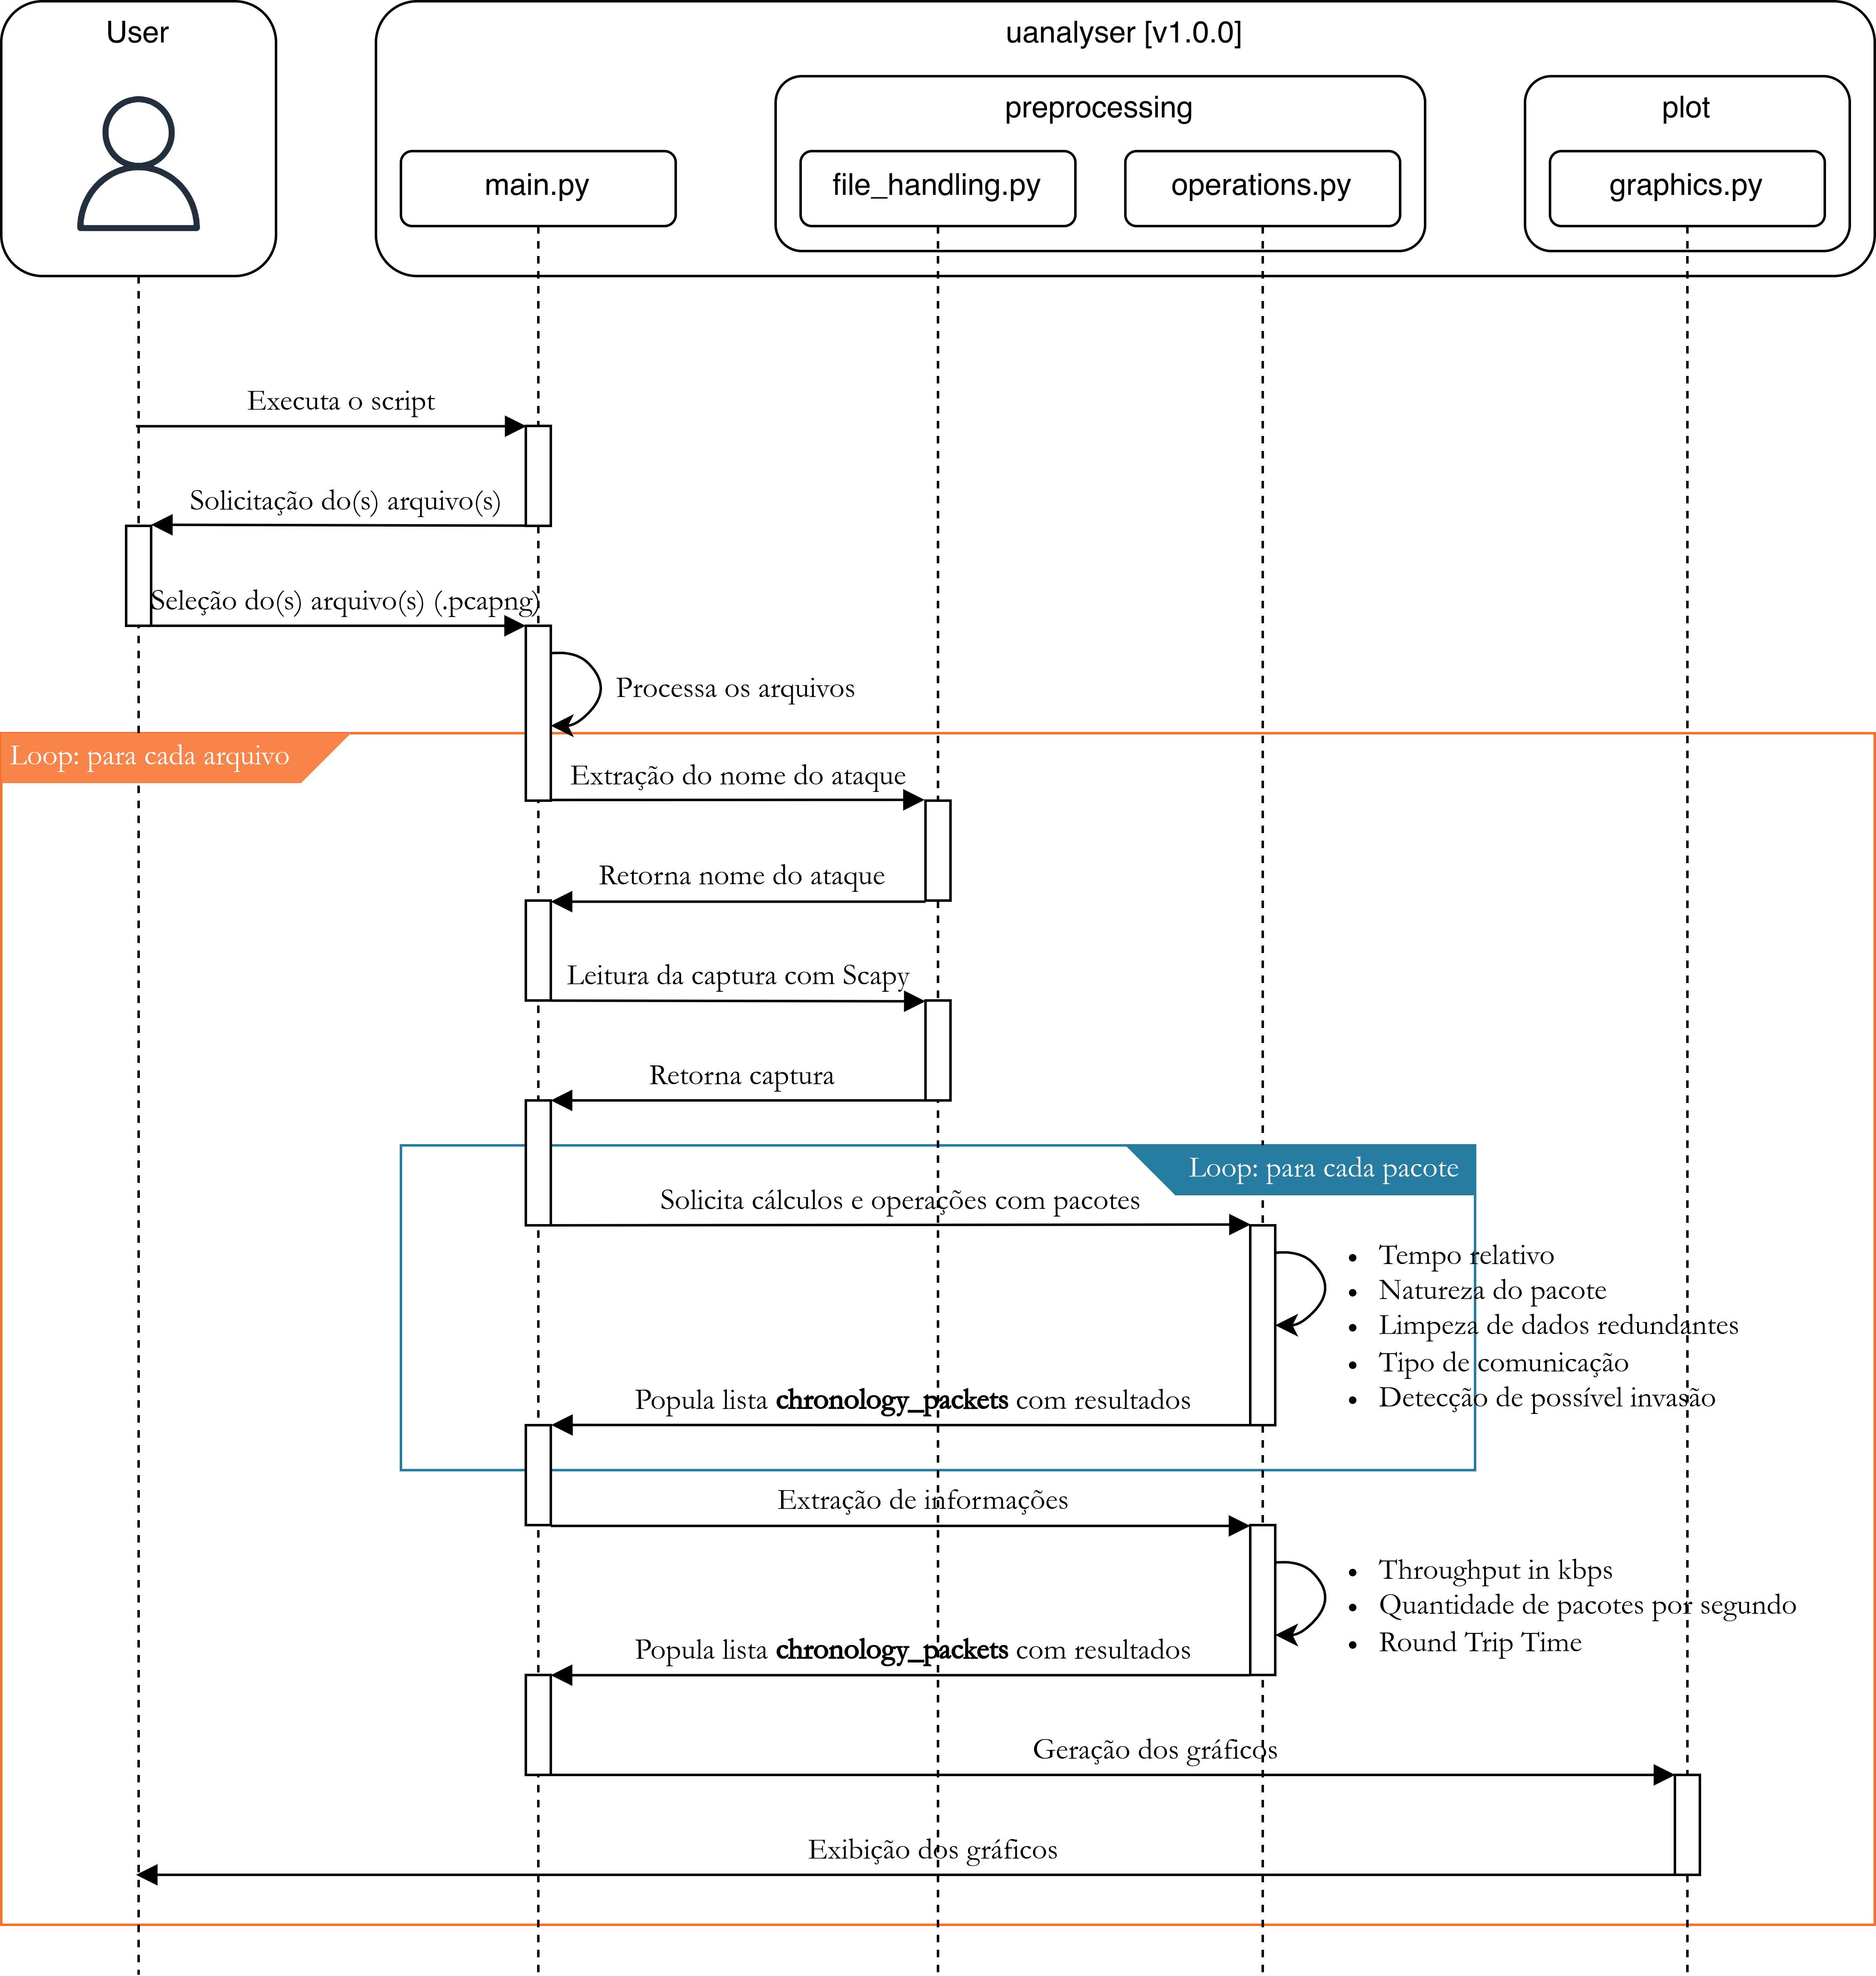
\includegraphics[width=0.972\textwidth]{USPSC-img/seqUanalyser.png}
            \end{center}
            \legend{Fonte: elaborada pelo autor.}
        \end{figure}

        Dentro do contexto do protocolo OPC UA, as mensagens trocadas entre cliente e servidor podem incluir várias estruturas de dados, como mensagens de sessão, mensagens de serviço e dados de publicação/subscrição. Cada tipo de mensagem possui seu próprio formato e estrutura, conforme especificado pelo padrão OPC UA. A análise dessas mensagens é fundamental para identificar comportamentos anômalos e potenciais vulnerabilidades.

        A análise dos pacotes capturados e a visualização dos gráficos gerados pelo \textbf{uanalyser} permitem uma compreensão detalhada dos efeitos dos ataques nas redes OPC UA. Essa abordagem sistemática e visual facilita a identificação de vulnerabilidades específicas do protocolo e o desenvolvimento de contramedidas eficazes para melhorar a segurança e a resiliência das redes industriais.

        O software desenvolvido para este trabalho está disponível no GitHub \footnote{Disponível em: \url{https://github.com/JonathanTSilva/opcua-analyser}. Acesso em: 04 jul. 2024} e aberto para contribuições. Aqueles que desejarem contribuir devem seguir os padrões de desenvolvimento estabelecidos no arquivo \texttt{contributing.md} e aderir ao código de conduta do projeto.

    \subsection{Análise dos Ataques e Vulnerabilidades}

        A análise de ataques e vulnerabilidades em redes industriais OPC UA é um processo sistemático e detalhado que visa identificar, avaliar e mitigar possíveis pontos fracos no protocolo e na implementação dessas redes. Essa etapa é essencial para garantir a segurança e a continuidade operacional dos IACS, consistindo na avaliação dos resultados de uma série de testes e simulações de ataques cibernéticos realizados nos processos anteriores. Cada tipo de ataque explora diferentes vulnerabilidades potenciais tanto do protocolo quanto da infraestrutura de rede.

        Ao testar as vulnerabilidades na comunicação de redes industriais OPC UA, o foco é determinar a qualidade da comunicação durante e após um ataque. Em outras palavras, verifica-se se o equipamento é capaz de desempenhar sua função nesses períodos. Além disso, examina-se se o alvo apresenta falta de resposta ou respostas incomuns.

        Como a observação de soluções existentes faz parte da abordagem deste desenvolvimento, é necessário ter um ponto de referência como base para a análise das vulnerabilidades e do comportamento durante os ataques. Com isso em mente, foram definidas as seguintes classes de vulnerabilidades para este projeto em específico:

        \begin{itemize}
            \item \textbf{Classe 1}: falhas que interrompem a comunicação OPC UA entre os agentes, afetando a disponibilidade;
            \item \textbf{Classe 2}: serviços interrompidos ou comportamento inesperado que não alteram a comunicação, mas comprometem a integridade;
            \item \textbf{Classe 3}: vulnerabilidades que não interrompem a comunicação, mas afetam a confiabilidade.
        \end{itemize}
        
        A partir dos gráficos gerados e da análise do comportamento da rede e dos dispositivos durante e após os ataques, é possível identificar as vulnerabilidades existentes e classificá-las conforme as classes mencionadas. Além disso, verifica-se a eficácia das diferentes políticas de segurança do OPC UA (`None', `Sign', `Sign \& Encrypt'). A análise dos resultados obtidos é fundamental para identificar possíveis falhas e propor medidas corretivas e preventivas, visando mitigar os riscos de segurança nas redes OPC UA.
        
        Essa abordagem metodológica, que inclui a observação de gráficos de throughput, desempenho de RAM e CPU, quantidade de pacotes OPC UA por segundo e RTT normalizado, permite uma compreensão detalhada do impacto dos ataques nas redes industriais OPC UA. Dessa forma, torna-se possível desenvolver estratégias de mitigação eficazes e assegurar a robustez e a resiliência das redes contra potenciais ameaças cibernéticas.
    
    \subsection{Relatório de Vulnerabilidade}

        A construção de um relatório de vulnerabilidade é uma etapa crucial no processo de avaliação da segurança cibernética, especialmente no contexto de redes industriais OPC UA. Por meio deste relatório, é possível documentar e comunicar as vulnerabilidades identificadas, fornecer uma análise detalhada dos riscos e propor contramedidas adequadas. Esse documento é fundamental não apenas para entender as falhas de segurança, mas também para tomar ações corretivas eficazes e melhorar a postura de segurança da organização.

        A elaboração de um relatório de vulnerabilidade deve seguir padrões internacionais de segurança cibernética e estar alinhada com as melhores práticas do setor. Um bom relatório deve ser estruturado de forma clara e objetiva, contemplando diferentes níveis de detalhamento para atender a diversos públicos, desde executivos até equipes técnicas.
        
        O relatório de vulnerabilidade é essencial para diversos stakeholders dentro de uma organização. Ele auxilia os executivos a compreenderem a postura de segurança atual da empresa e a justificarem investimentos na área. Para a equipe de TI, o relatório oferece detalhes técnicos sobre as vulnerabilidades descobertas e orientações sobre como corrigi-las. Além disso, o relatório pode ser utilizado para fins de conformidade regulatória, sendo compartilhado com auditores e reguladores para demonstrar os esforços de segurança da organização.
        
        Para garantir a eficácia do relatório de vulnerabilidade, ele deve incluir as seguintes seções principais:

        \begin{itemize}
            \item \underline{Sumário Executivo}: Uma visão geral de alto nível da avaliação, destinada a executivos não técnicos. Esta seção deve auxiliar os executivos na avaliação da postura de segurança da empresa, destacando quaisquer questões críticas que possam impactar a segurança corporativa ou a conformidade regulatória.
            \item \underline{Visão Geral}: Seção voltada para um público mais técnico, que oferece um resumo da avaliação. Deve incluir informações sobre os sistemas analisados, ferramentas utilizadas, além do número e da severidade das vulnerabilidades descobertas.
            \item \underline{Detalhes da Avaliação}: Esta seção deve fornecer informações técnicas detalhadas sobre como a avaliação de vulnerabilidades foi conduzida. Deve descrever as etapas realizadas em cada fase da avaliação e seus resultados, permitindo que o leitor possa replicar os achados.
            \item \underline{Resultados}: Esta seção deve detalhar os achados da avaliação. As vulnerabilidades devem ser classificadas por severidade, destacando os maiores problemas no ambiente da organização. Para cada vulnerabilidade verificada, deve-se descrever o resultado, os sistemas afetados, o nível de severidade e fornecer um link para informações adicionais, como um CVE.
            \item \underline{Mitigações Recomendadas}: O objetivo de uma avaliação de vulnerabilidades é auxiliar a organização a melhorar sua postura de segurança. Portanto, fornecer recomendações de mitigação é essencial. Em muitos casos, isso pode ser tão simples quanto recomendar uma atualização de software, uma senha mais forte em um sistema, ou a alteração de uma configuração de segurança insegura.
        \end{itemize}

        Uma vez que o relatório de vulnerabilidade é elaborado, ele deve ser incorporado às bases de conhecimento da organização para garantir que todas as vulnerabilidades identificadas sejam tratadas de forma adequada. O relatório deve ser revisado regularmente e atualizado conforme novas vulnerabilidades forem descobertas e medidas corretivas forem implementadas. Além disso, é importante que o relatório siga os padrões globais de cibersegurança, como o CVE (\textit{Common Vulnerabilities and Exposures}) e as normas de segurança IEC 62443, para assegurar a consistência e a confiabilidade das informações.

        A adoção de frameworks reconhecidos internacionalmente, como o CVE e o IEC 62443, proporciona uma base sólida para a identificação e classificação de vulnerabilidades. Esses padrões oferecem diretrizes claras sobre como avaliar e mitigar riscos, além de promover práticas de segurança consistentes e eficazes. Adicionalmente, existem diversos modelos para a elaboração de relatórios de vulnerabilidade, como os da CISA (Cybersecurity and Infrastructure Security Agency) e do NIST (National Institute of Standards and Technology), que podem ser adaptados para atender às necessidades específicas de cada organização. Caso alguma vulnerabilidade desconhecida no protocolo OPC UA seja encontrada, será utilizado um modelo de relatório personalizado, disponível no \autoref{ap:relatorio}, para documentar e comunicar a descoberta.

    \subsection{Contramedidas de Segurança}

        Uma implementação bem projetada e descomplicada das contramedidas de segurança é uma das principais estratégias para minimizar os riscos cibernéticos e maximizar a disponibilidade dos IACS. A segurança das redes industriais OPC UA deve adotar uma abordagem holística, que inclua a proteção dos ativos de informação, a prevenção de ameaças e a detecção de incidentes.

        A determinação das contramedidas varia de acordo com o cenário de ataque e as vulnerabilidades identificadas. No entanto, algumas práticas comuns podem ser adotadas para fortalecer a segurança das redes OPC UA. Entre as principais contramedidas recomendadas estão:

        \begin{itemize}
            \item \underline{Criptografia e modos de segurança:} conforme recomendado pelas políticas de segurança `Sign' e `Sign \& Encrypt', a criptografia e a assinatura da comunicação OPC UA se destacam como as principais melhorias na configuração de segurança. Isso inclui a utilização de certificados robustos e algoritmos de criptografia atualizados.
            \item \underline{Alto nível de autenticação:} implementação de métodos de autenticação forte para acesso ao servidor OPC UA, incluindo autenticação multifator (MFA) e uso de certificados digitais para a autenticação de dispositivos.
            \item \underline{Aprimoramento da segurança da rede:} criação de zonas de segurança dentro da rede industrial para limitar a propagação de ataques, seguindo o modelo de defesa em profundidade (\textit{defense in depth}), no qual cada zona é separada por \textit{firewalls} e dispositivos de segurança que monitoram e controlam o tráfego de rede. O modelo \textit{Zero Trust} é uma abordagem complementar à segregação de rede, operando sob a premissa de "nunca confiar, sempre verificar". Este modelo considera a rede como inerentemente insegura e requer autenticação e autorização rigorosas para cada tentativa de acesso.
            \item \underline{Controle de Acesso Baseado em Função (RBAC, do inglês \textit{Role-Based Access Control}):} aplicado para limitar o acesso aos recursos de rede e serviços de comunicação apenas a usuários e dispositivos autorizados, minimizando o risco de acessos não autorizados.
            \item \underline{Monitoramento contínuo:} implementação de sistemas de monitoramento contínuo para detectar atividades anômalas e potenciais ataques em tempo real. IDS (\textit{Intrusion Detection Systems}) e SIEM (\textit{Security Information and Event Management}) são sistemas eficazes utilizados para garantir esse diagnóstico contínuo.
            \item \underline{Resposta a incidentes:} um plano de resposta a incidentes bem elaborado, que define procedimentos claros para identificar, conter e remediar ataques cibernéticos, é imprescindível para mitigar possíveis ameaças às redes industriais. Este plano pode ser baseado nas melhores práticas recomendadas pela norma IEC 62443 e frameworks de segurança correlatos.
            \item \underline{Atualizações regulares:} garantia de que todos os componentes da rede, incluindo o servidor OPC UA e dispositivos de rede, estejam sempre atualizados com os últimos \textit{patches} de segurança.
            \item \underline{\textit{Hardening} de sistemas:} aplicação de técnicas de \textit{hardening} para reduzir a superfície de ataque do servidor e dos dispositivos de rede. Isso inclui a desativação de serviços desnecessários, configuração segura de sistemas operacionais e aplicações, e implementação de políticas de segurança rigorosas.
        \end{itemize}

        A determinação e implementação de contramedidas de segurança em redes industriais OPC UA é um processo complexo, mas essencial para garantir a segurança e a integridade dos sistemas de automação e controle. Por meio da combinação de uma análise detalhada de vulnerabilidades, referência a frameworks de segurança reconhecidos e avaliação contínua da eficácia das medidas implementadas, é possível desenvolver uma abordagem robusta para proteger redes OPC UA contra uma ampla gama de ameaças cibernéticas. Este trabalho contribui para o fortalecimento da segurança nas redes industriais, promovendo a resiliência dos sistemas críticos em um cenário de ameaças em constante evolução.